\documentclass[a4paper,12pt]{book}
\usepackage[T2A]{fontenc}
\usepackage[utf8]{inputenc}
\usepackage[russian]{babel}
\usepackage[utf8]{inputenc}
\usepackage{pscyr}          % Нормальные шрифты
\usepackage{graphicx,xcolor}

\usepackage[left=2cm,right=2cm,top=2cm,bottom=2cm,bindingoffset=0cm]{geometry}
\usepackage{wrapfig}   % обтекаемые текстом блоки
\usepackage{soulutf8}  % выделение текста
\usepackage{xcolor}    % выделение цветом
\usepackage{array}
\usepackage{booktabs}
\usepackage{multirow,bigdelim}
\usepackage{hhline}
\usepackage{tabularx}
\usepackage{hyperref}
\usepackage{amsmath,amssymb}
\usepackage{nccboxes}
\usepackage{mathtext}
\usepackage{floatflt}
\usepackage{textcomp}

\hypersetup{pdftitle={Электромагнитные переходные процессы}}  % метаданные PDF
\hypersetup{pdfauthor={Сергей Александрович Ульянов}}
\hypersetup{pdfcreator={LaTeX}}
\hypersetup{pdfproducer={http://ulianov.net}}


\hypersetup{ pdfborder={0 0 0}} % раскомментировать, чтобы ссылки не выделялись
%\renewcommand{\theenumi}{(\Asbuk{enumi})}

% Этот код нужен для конвертации svg в pdf+tex на лету, взято из
% http://mirrors.ctan.org/info/svg-inkscape/InkscapePDFLaTeX.pdf
\graphicspath{{pic/}} 
\newcommand{\executeiffilenewer}[3]{
	\ifnum\pdfstrcmp{\pdffilemoddate{#1}}
	{\pdffilemoddate{#2}} > 0 {\immediate\write18{#3}}\fi}
\newcommand{\includesvg}[1]{
	\executeiffilenewer{#1.svg}{#1.pdf}
	{inkscape -z -D --file=#1.svg --export-pdf=#1.pdf --export-latex --export-png=#1.png}
	\input{#1.pdf_tex}%
}

%-----------------------------------

\begin{document}

\author{Сергей Александрович Ульянов}
\title{Электромагнитные переходные процессы}
\date{1970}

\frontmatter
\maketitle
\tableofcontents
\mainmatter

\chapter*{Предисловие}
\addcontentsline{toc}{chapter}{Предисловие}
\label{chap:0 preface}

Предлагаемая книга является учебником по первой части курса «Переходные процессы в электрических системах», в которой рассматриваются только электромагнитные переходные процессы.

Она написана в соответствии с программой по данному курсу (инд. У-Т-3/160), утвержденной Учебно-методическим Управлением MB и ССО СССР в 1968~г. для специальностей: «Электрические станции» (0301), «Электрические системы и сети» (0302) и «Кибернетика электрических систем» (0304). С некоторыми сокращениями она, очевидно, может быть использована и для других электротехнических специальностей и специализаций.

Весь материал книги разбит на четыре раздела; при этом в четвертый раздел отнесены \colorbox{red}{гл.~16--19} которые между собой не связаны.

При построение книги автор опирался преимущественно на свой многолетний опыт преподавания данного курса в Московском ордена Ленина энергетическом институте. Следует отметить, что не весь материал подлежит изложению на лекциях. Так, например, содержание гл.~\ref{chap:2 obshchie ukazaniia k vypolneniiu raschetov} почти полностью целесообразно прорабатывать на практических занятиях. К тому же, это в сущности вынужденное решение, так как лектор не успевает, прочитать все, что нужно к первому практическому занятию.

В зависимости от местных условий и обстоятельств (как-то: наличие лаборатории по курсу и ее пропускной способности и пр.) в рабочем календарном плане иногда приходится менять порядок прохождения отдельных тем, добиваясь наибольшей согласованности с тематикой практических занятий и содержанием каждого этапа заданий, которые самостоятельно выполняют студенты. Для этого основы строгой теории переходных процессов и ее применение (гл. \colorbox{red}{7—9}) лектор обычно вынужден излагать после практических методов расчета (гл. \colorbox{red}{10}). Равным образом более подробное знакомство с гл. \colorbox{red}{13} приходится давать после гл. \colorbox{red}{14} и \colorbox{red}{15}. Однако сделать такую перестановку в учебнике было бы неправильным, так как местные условия могут быть весьма различны, а кроме того, учебником пользуются учащиеся, которые не ограничены подобными рамками (например, студенты-заочники).

Несмотря на то что недавно вышел в свет сборник задач по данной части курса, автор не счел возможным ограничиться малым числом примеров. Все принципиальные вопросы и методы расчета в книге иллюстрированы необходимым количеством примеров, в которых приведены подробные решения.

Автор надеется; что эта книга найдет своих читателей также среди инженерно-технических работников и принесет им пользу в их практической деятельности.

При создании данной книги автор использовал не только свои работы, но также многочисленные работы по исследованию и расчету электромагнитных переходных процессов, выполненные в Советском Союзе: А.~А.~Горева, Н.~Н.~Щедрина, Д.~А.~Городского, Н.~Ф.~Марголина, Л.~Г.~Мамиконянца, И.~М.~Марковича, А.~Б.~Чернина и др. и за рубежом: Р.~Рюденберга, К.~Парка, Э.~Кларк, К.~Вагнера, Р.~Эванса, Э.~Кимбарка, К.~Ковача, И.~Раца и др. Поскольку книга предназначена для учебных целей, не представляется возможным всюду давать ссылки на первоисточники. Помещенный в конце книги перечень литературы ориентирован в основном на интересы и возможности студентов. Более полный, но далеко не исчерпывающий список литературы приведен в книге автора, изданной в 1964~г. \cite{04Ulianov64}.

Автор выражает глубокую благодарность коллективу кафедры «Электрические станции, сети и системы» Рижского политехнического института и доктору техн. наук, шроф. Н.~И.~Соколову за рецензирование рукописи и сделанные ими замечания и предложения, которые учтены при окончательной подготовке рукописи к печати.

С благодарностью автор отмечает большую работу канд. техн. наук, доц. И.~П.~Крючкова по тщательному редактированию рукописи.

Все замечания и пожелания по данной книге автор примет с (признательностью и просит их направлять в адрес издательства «Энергия» (Москва, Ж-114, Шлюзовая наб., 10).

\vspace{1pc}
\begin{minipage}{0.49\linewidth}
	Москва, 1970
\end{minipage}
\hfill
\begin{minipage}{0.49\linewidth}
	\flushright
	\textit{С.~А.~Ульянов}
\end{minipage}

\chapter*{Введение}
\addcontentsline{toc}{chapter}{Введение}
\label{chap:0 intro}

Курс «Переходные процессы в электрических системах» является одним из профилирующих для электроэнергетических специальностей и специализаций.

Переходные процессы возникают в электрических системах как при нормальной эксплуатации (включение и отключение нагрузок, источников питания, отдельных цепей, производство испытаний и пр.), так и в аварийных условиях (обрыв нагруженной цепи или отдельной ее фазы, короткое замыкание, выпадение машины из синхронизма и т.~д. Их изучение, разумеется, не может быть самоцелью. Оно необходимо прежде всего для ясного представления причин возникновения и физической сущности этих процессов, а также дли разработки практических критериев и методов их количественной оценки, с тем чтобы можно было предвидеть и заранее предотвратить опасные последствия таких процессов. Короче говоря, важно понимать переходные процессы, но еще важнее уметь сознательно управлять ими.

При любом переходном процессе происходит в той или иной мере изменение электромагнитного состояния элементов системы и нарушение баланса между моментом на валу каждой вращающийся машины и электромагнитным моментом.

В результате этого нарушения соответственно изменяются скорости вращения машин, т.~е. некоторые машины испытывают торможение, в то время как другие --- ускорение. Такое положение существует до тех пор, пока регулирующие устройства не восстановят нормальное состояние, если это вообще осуществимо при изменившихся условиях.

Из сказанного следует, что переходный процесс характеризуется совокупностью электромагнитных и механических изменений в системе. Последние взаимно связаны и по существу представляют единое целое. Тем не менее благодаря довольно большой механической инерции вращающихся машин начальная стадия переходного процесса характеризуется преимущественно электромагнитными изменениями. В самом деле, вспомним хотя бы процесс пуска асинхронного двигателя. С момента включения его в сеть до момента начала разворота ротора двигателя имеет место только электромагнитный переходный процесс, который затем дополняется механическим переходным процессом. Процесс пуска двигателя значительно усложняется, если учесть возникающую реакцию источника питания и действие его автоматических регулирующих устройств.

При относительно малых возмущениях (например, при коротком замыкании за большим сопротивлением или, как говорят, при большой удаленности короткого замыкания) весь переходный процесс практически можно рассматривать только как электромагнитный. Для иллюстрации укажем, что в установке с напряжением 400~\textit{в} ток короткого замыкания в 5000~\textit{а} после его приведения к стороне генераторного напряжения составляет менее 1,5\% номинального тока современного турбогенератора 200~\textit{Мвт}(15,75~\textit{кв}). Естественно, такое малое увеличение тока не вызовет заметного нарушения равновесия рабочего состояния упомянутого турбогенератора.

Таким образом, при известных условиях представляется возможным и целесообразным рассматривать только одну   сторону переходного процесса, а именно явления электромагнитного характера. В  соответствии с этим настоящий курс разбит на две части. В первой из них рассматриваются электромагнитные переходные процессы\footnote{В конце первой части рассматривается упрощенный учет качаний генераторов, что является естественным переходом ко второй части курса.}, а во второй --- совместно электромагнитные и механические, т.~е. электромеханические переходные процессы. Такое деление помогает учащемуся постепенно осваивать разнообразный и достаточно сложный материал курса.

При провождении курса «Теоретические основы электротехники» читатель уже знакомился с переходными процессами в цепях с сосредоточенными и распределенными параметрами. Рассмотрение этих процессов проводилось в предположении, что цепь является однофазной и ее питание осуществляется от источника с заранее известным напряжением (как по величине, так и по закону его изменения). В данном курсе предстоит рассмотреть более сложные задачи, когда переходный процесс возникает в многофазной цепи, при этом он одновременно протекает в самих источниках питания, у которых дополнительно приходят в действие автоматические регулирующие устройства. В этом случае напряжения всех источников\footnote{За исключением тех, мощность которых практически может быть принята бесконечно большой.} являются неизвестными переменными величинами.

Преподавание в вузах этого курса как самостоятельной специальной дисциплины\footnote{Точнее, двух дисциплин,  так как вначале читались отдельно курс коротких замыканий и курс устойчивости электрических систем.} началось в конце 20-х годов. За истекшее время его содержание и число часов, отводимое на него в учебных планах, неоднократно менялось. В последние годы установлена более тесная последовательная связь между его обеими частями.

Первая часть данного курса использует материал, изученный в курсах высшей математики (операционное исчисление), теоретических основ электротехники (линейные цепи), электрических машин (преимущественно синхронные и асинхронные машины) и электрических сетей и систем.

В свою очередь материал первой части данного курса используется при прохождении его второй части, а также при дальнейшем изучении других специальных курсов, как-то: электрических систем, дальних передач, основного электрооборудования станций, техники релейной защиты, автоматизации электрических систем и др.

Практические задачи, при решении которых инженер-электрик сталкивается с необходимостью количественной оценки тех или иных величин во время электромагнитного переходного процесса, многочисленны и разнообразны (см.~§\ref{sec:1-3 naznacheniia_raschetov_i_trebovaniia_k_nim}). Однако все они в конечном итоге объединены единой целью обеспечить надежность работы отдельных элементов и электрической системы в целом.

Теперь сделаем небольшую экскурсию в прошлое и покажем вкратце как развивалась проблема переходных процессов преимущественно в части исследования электромагнитных переходных процессов.

В то время как теория установившихся режимов развивалась в правильном направлении и быстро приспособилась к нуждам практики, сущность переходных процессов долго оставалась невыясненной. На примере развития электромашиностроения нетрудно проследить, насколько важен учет явлений, в частности, при коротких замыканиях.

Первоначальные конструкции электрических машин выполнялись лишь в соответствии с требованиями нормальной работы. Пока мощности машин были малы, их конструкции обладали как бы естественным запасом устойчивости против механических и тепловых действий токов короткого замыкания. Однако такое положение существовало недолго. По мере роста мощности машин и особенно после осуществления их параллельной работы размер повреждений машин при коротких замыканиях резко возрос. Становилось очевидным, что нельзя обеспечить надежную конструкцию машины, не считаясь с аварийными условиями работы. Успех предлагаемых мер по усилению конструкций зависел от достоверности знаний самого процесса короткого замыкания. Так постепенно создавались все более совершенные конструкции электрических машин. В современном исполнении они являются одним из надежных элементов систем. Разумеется, эта надежность достигнута при учете и других опасных условий, в которых может оказаться машина.

Аналогичное положение наблюдалось при поисках способов гашения магнитного поля электрических машин. Недостаточность первоначальных сведений об этом процессе приводила к малоэффективным решениям. Подобные примеры можно обнаружить и в других областях электроэнергетики (аппаратостроении, технике релейной защиты и др.).

Более серьезная разработка теории переходных процессов в электрических машинах началась с первых лет текущего столетия. В конце 20-х годов Парк (Park) разработал строгую теорию переходных процессов в электрических машинах, приняв в основу ранее предложенную Блонделем (Blondel) теорию двух реакций. Эта теория обеспечила быстрое развитие дальнейших исследований в данной области. Они интенсивно проводились у нас в Союзе и за рубежом, главным образом в США. Особое место среди них занимают работы А.~А.~Горева.

Примерно в те же годы стала находить все более широкое применение теория симметричных составляющих, остававшаяся в течение нескольких лет без использования. Она позволила решить на строгой научной основе все вопросы, связанные с несимметрией в многофазной цепи.

Наряду с теоретическими исследованиями существенно важной являлась своевременная разработка практических методов расчета переходных процессов. В этом испытывалась острая нужда в связи с проводившейся широкой электрификацией нашей страны.

К выполнению таких работ привлекались научно-исследовательские и учебные институты (ВЭИ, МЭИ, ЛПИ, ХЭТИ и др.), крупные энергообъединения (Мосэнерго, Ленэнерго) и проектные организации (ТЭП). Для координации работ, обобщения результатов, подготовки решений и рекомендаций были созданы специальные комиссии. Так, в 30-х годах под председательством К.~А.~Круга работала комиссия по разработке указаний к выполнению расчетов коротких замыканий.

Теоретические исследования и практические методы расчета всегда требуют экспериментальной проверки. Ранее ее проводили в натуральных условиях. Однако испытания проводились крайне редко из-за значительного риска, что такой эксперимент повлечет серьезную аварию, поскольку системы не располагали достаточным резервом мощности, связи между станциями были слабы, отсутствовали многие автоматические устройства (как-то: регулирование возбуждения генераторов, повторное включение цепей и др.) и, наконец, само оборудование было еще недостаточно совершенным (например, время действия выключателей составляло десятые доли секунды). Позже и особенно в последнее время благодаря значительному усовершенствованию электрических систем подобные эксперименты проводят по мере надобности, причем, как правило, они не вызывают каких-либо заметных помех в нормальной работе системы. С той же целью используются записи автоматических осциллографов, которыми все больше оснащают наиболее ответственные и характерные цепи систем.

Неоценимую помощь в экспериментировании и проверке ряда новых теоретических разработок, схем и автоматических устройств оказало и продолжает оказывать физическое и математическое моделирование электрических систем. Применение электронных вычислительных машин непрерывного действия (машины-аналоги) и дискретного действия (цифровые машины) в значительной мере расширили возможности очень эффективного математического моделирования.

Расчетные модели, где все элементы системы (включая генераторы) представлены схемами замещения, уже свыше 35~лет широко используют для решения многих задач. В зависимости от их конструкции они позволяют получить решение в соответствии с принятым методом расчета, почти полностью освобождая от утомительной и трудоемкой вычислительной работы, что также очень ценно.

По вопросам переходных процессов в электрических системах, их моделированию и практическим методам их расчета написано много книг. Лишь некоторые из них указаны в данном учебнике.
\chapter{Основные сведения об электромагнитных переходных процессах}
\label{chap:1 osnovnye_svedeniia_ob_elektromagnitnykh_perehodnykh_protcessakh}

\section{Основные определения}
\label{sec:1-1 osnovnye_opredeleniia}

Из всего многообразия электромагнитных переходных процессов в электрической системе наиболее распространенными являются процессы, вызванные:
\begin{enumerate} 
	\item
	включением и отключением двигателей и других приемников электроэнергии;
	\item
	коротким замыканием в системе, а также повторным включением и отключением (одновременным или 
каскадным) короткозамкнутой цепи;
	\item
	возникновением местной несимметрии в системе (например, отключение одной фазы линии передачи);
	\item
	несинхронным включением синхронных машин. 
\end{enumerate}

\so{Коротким замыканием} называют всякое не предусмотренное нормальными условиями работы замыкание между фазами, а в системах с заземленными нейтралями (или четырехпроводных)~---  также замыкание одной или нескольких фаз на землю (или на нулевой провод).

В системах с незаземленными нейтралями или с нейтралями, заземленными через специальные компенсирующие устройства, замыкание одной из фаз на землю называют \so{простым замыканием}. При этом виде повреждения прохождение тока обусловлено главным образом емкостью фаз относительно земли.

При возникновении короткого замыкания в электрической системе сопротивление цепи уменьшается (степень уменьшения зависит от положения точки короткого замыкания в системе), что приводит к увеличению токов в отдельных ветвях системы по сравнению с токами нормального режима. в свою очередь это вызывает снижение напряжений в системе, которое особенно велико вблизи места короткого замыкания.

Обычно в месте замыкания образуется некоторое переходное сопротивление, состоящее из сопротивления возникшей электрической дуги и сопротивлений прочих элементов пути тока от одной фазы к другой или от фазы на землю. Электрическая дуга возникает или с самого начала происшедшего повреждения как, например, при перекрытии или пробое изоляции, или через некоторое время, когда перегорит элемент, вызвавший замыкание. При замыканиях между фазами переходное сопротивление определяется главным образом сопротивлением электрической дуги.

\begin{wrapfigure}[17]{r}{0.4\linewidth} % 1-1
	\centering
	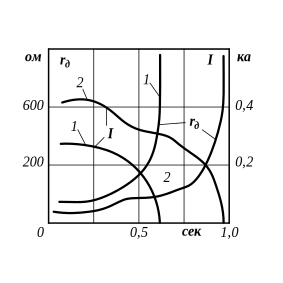
\includegraphics[width=0.95\linewidth]{pic/1-1}
	\caption{Кривые изменения во времени тока и сопротивления самопогасающей открытой дуги на линии 110~\textit{кв} с деревянными опорами. \textit{1, 2} -- номера опытов.}
	\label{fig:1-1 r_i_I}
\end{wrapfigure}


Когда токи достаточно велики (сотни ампер и более), сопротивление дуги приблизительно постоянно и по своему характеру почти чисто активное. С уменьшением, тока и увеличением длины дуги, что имеет место в течение переходного процесса, ее сопротивление возрастает. Наглядной иллюстрацией такого изменения могут служить графики (рис.~\ref{fig:1-1 r_i_I}), полученные экспериментально при возникновении самопогасающих дуг на линиях 110~\textit{кв} с деревянными опорами.

В ряде случаев переходные сопротивления могут быть столь малы, что практически ими можно пренебречь. Такие замыкания называют \so{металлическими}.

Естественно, при прочих равных условиях ток при металлическом замыкании больше, чем при наличии переходного сопротивления. Поэтому, когда требуется найти возможные наибольшие величины токов, исходят из наиболее тяжелых условий, считая, что в месте замыкания отсутствуют какие-либо переходные сопротивления\footnote{Учет переходных сопротивлений и контактных соединений при выполнении расчетов коротких замыканий для установок напряжением до 1000~\textit{в} имеет особое значение (\colorbox{red}{§~17-5}).}.

В трехфазных системах с заземленной нейтралью различают следующие основные виды коротких замыканий в одной точке:

\begin{enumerate} 
	\item
	трехфазное;
	\item
	двухфазное;
	\item
	однофазное;
	\item
	двухфазное на землю, т.~е, замыкание между двумя фазами с одновременным замыканием той же точки на землю. 
\end{enumerate}

Трехфазное короткое замыкание является симметричным, так как при нем все фазы остаются в одинаковых условиях\footnote{При наличии переходных сопротивлений симметрия сохраняется лишь при равенстве этих сопротивлений.} Напротив, все остальные виды коротких замыканий являются несимметричными, поскольку при каждом из них фазы находятся уже в неодинаковых условиях; поэтому системы токов и напряжений при этих видах короткого замыкания в той или иной мере искажены.
	
Многолетняя аварийная статистика по союзным и зарубежным системам показывает, что при глухозаземленной нейтрали относительная вероятность различных основных видов короткого замыкания характеризуется примерными данными табл. \ref{tabl:1-1 veroiatnost_kz} В той же таблице показаны рекомендуемые сокращенные обозначения каждого вида короткого замыкания.

Как видно из этой таблицы, подавляющее число коротких замыканий связано с замыканием на землю, в то время как трехфазное короткое замыкание является очень редким. Однако отсюда было бы неправильным делать вывод, что трехфазное короткое замыкание можно вообще оставить без внимания. Поскольку оно все же возможно, с ним следует считаться, тем более что оно иногда может быть решающим для окончательного суждения относительно возможности работы в условиях короткого замыкания. Само изучение процесса трехфазного короткого замыкания особенно важно в связи с тем, что применение метода симметричных составляющих позволяет величины токов и напряжений прямой последовательности любого несимметричного замыкания определять как соответственные величины при некоторых условных трехфазных замыканиях.

\begin{table}[h] % 1-1
	\centering
	\begin{tabular}{|>{\centering\arraybackslash}m{0.2\linewidth}|>{\centering\arraybackslash}m{0.32\linewidth}|>{\centering\arraybackslash}m{0.19\linewidth}|>{\centering\arraybackslash}m{0.19\linewidth}|}
		\hline
		Виды короткого замыкания & Принципиальная схема & Буквенное обозначение на схемах места и вида короткого замыкания & Относительная вероятность короткого замыкания, \% \\
		\hline
		Трехфазное & 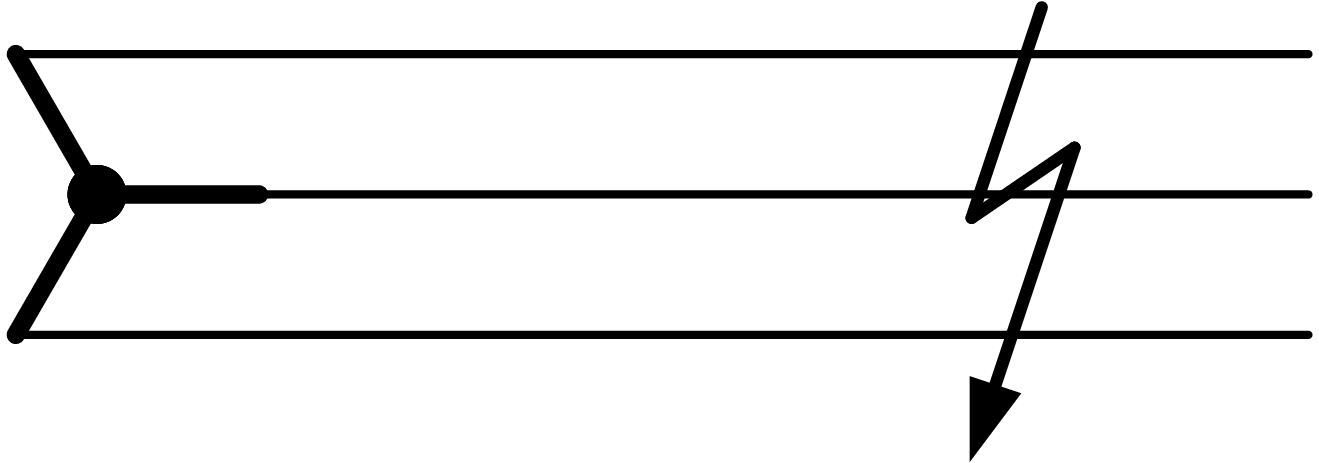
\includegraphics[width=0.7\linewidth]{pic/1-x-1} & $ K^{(3)} $ & 5 \\
		Двухфазное & 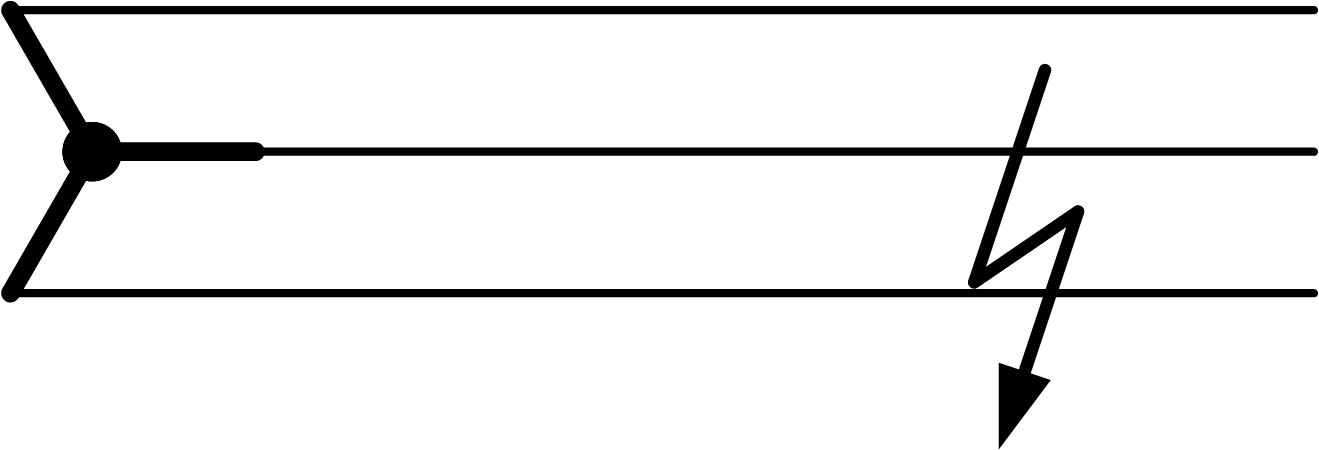
\includegraphics[width=0.7\linewidth]{pic/1-x-2} & $ K^{(2)} $ & 10 \\
		Однофазное & 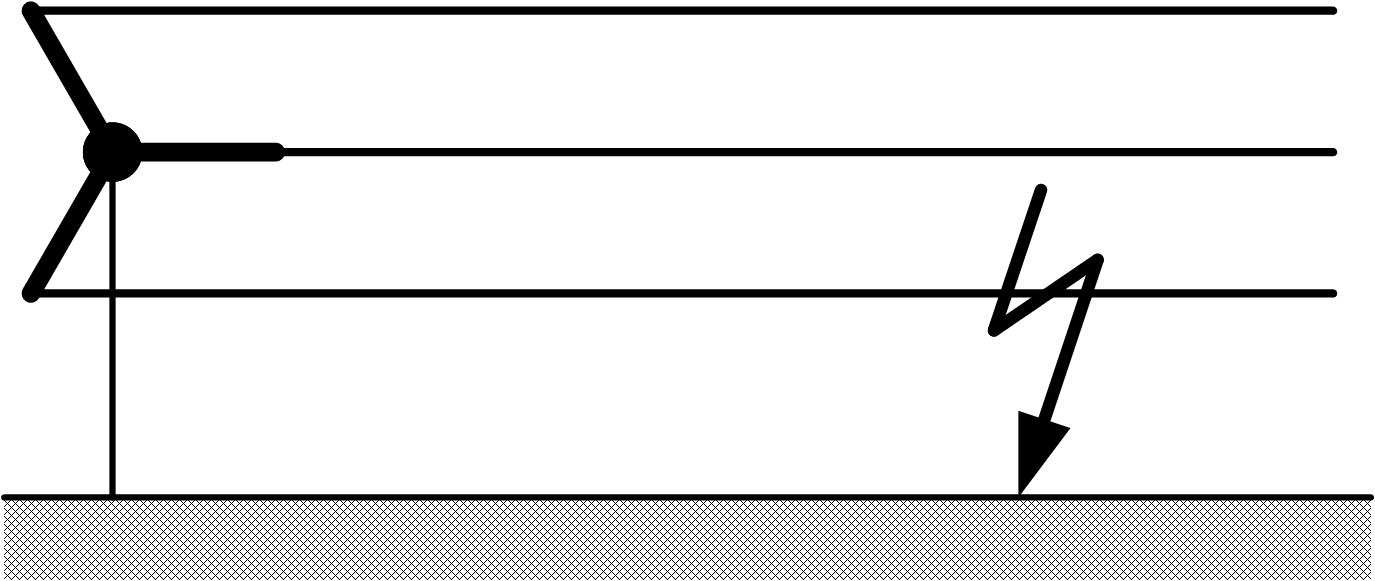
\includegraphics[width=0.7\linewidth]{pic/1-x-3} & $ K^{(1)} $ & 65 \\
		Двухфазное на землю & 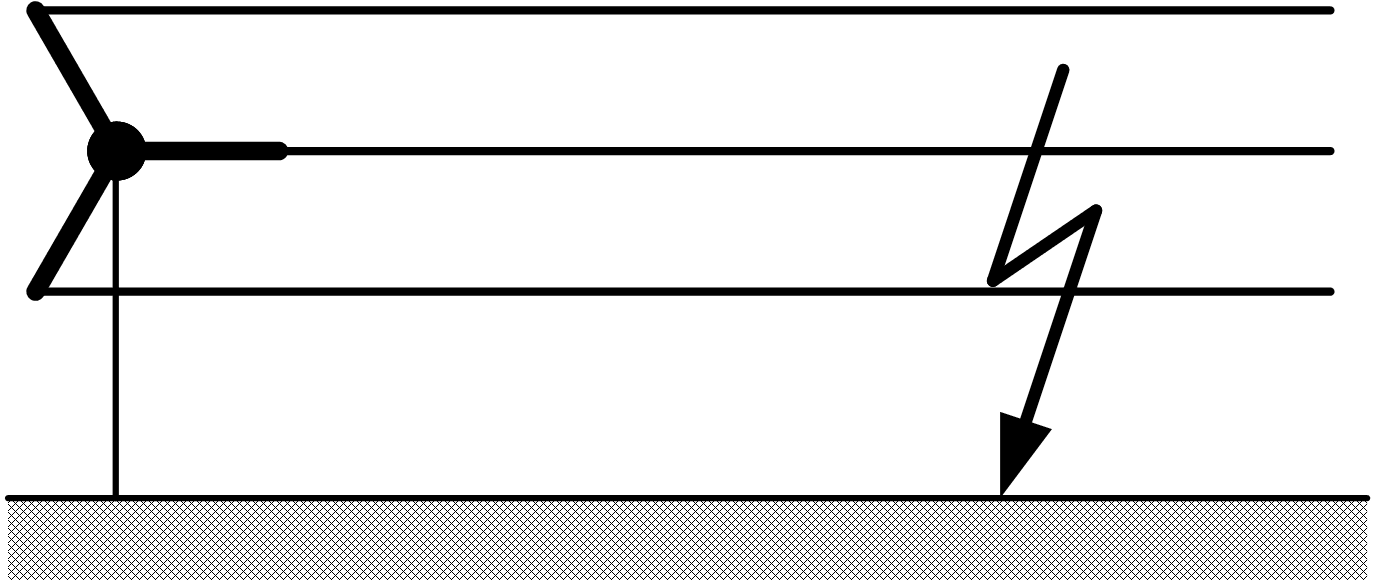
\includegraphics[width=0.7\linewidth]{pic/1-x-4} & $ K^{(1,1)} $ & 20 \\
		\hline
	\end{tabular}
	\caption{Относительная вероятность и сокращенные обозначения основных видов короткого замыкания}
	\label{tabl:1-1 veroiatnost_kz}
\end{table}

Здесь нелишне также отметить, что процесс включения любого трехфазного приемника или невозбужденного синхронного генератора или двигателя можно рассматривать как трехфазное короткое замыкание за некоторым сопротивлением.

Иногда в процессе развития аварии первоначальный вид короткого замыкания переходит в другой вид короткого замыкания. Так, например, в кабельных сетях (с трехжильными кабелями) несимметричные короткие замыкания часто переходят в трехфазные короткие замыкания, так как образовавшаяся при повреждении в кабеле электрическая дуга быстро разрушает изоляцию между его жилами.

Несимметричные короткие замыкания, а также несимметричные нагрузки по существу представляют различные виды \so{поперечной несимметрии}.

Нарушение симметрии какого-либо промежуточного элемента трехфазной цепи (например, отключение одной фазы линии передачи и т.~п.) называют \so{продольной несимметрией}.

Возможны случаи, когда одновременно возникает несколько несимметрий одинакового или различного вида. Так, например, при обрыве провода воздушной линии один его конец, расположенный близко к точке подвеса, остается изолированным, а другой, упав на землю, образует однофазное короткое замыкание. Здесь одновременно возникают продольная и поперечная несимметрии. В качестве другого примера, когда возникают несимметрии одного вида, может служить так называемое \so{двойное замыкание на землю}, т.~е. одновременное замыкание на землю разных фаз в различных точках сети, работающей с изолированной нейтралью.

Все виды повреждений, сопровождающихся мног кратной несимметрией, называют \so{сложными}. К ним, очевидно, относится также любое несимметричное короткое замыкание в сети, работающей в неполнофазном режиме.

Практикой эксплуатации электрических систем установлено, что большая часть возникающих повреждений, особенно на воздушных линиях, имеет проходящий характер, т.~е. повреждения самоустраняются после отключения поврежденного участка и не возникают вновь при обратном включении его. Примером такого самоустраняющегося повреждения может служить обычное перекрытие по поверхности гирлянды изоляторов линии, вызванное грозовым разрядом. После отключения линии электрическая прочность воздушного промежутка восстанавливается в течение небольшого отрезка времени, необходимого для деионизации воздуха в месте перекрытия.

В соответствии с этим широкое применение нашло автоматическое повторное включение (АПВ) цепей и особенно воздушных линий. Поскольку на последних преобладают замыкания одной фазы, у них производят иногда отключение только поврежденной фазы с после дующим однофазным автоматическим повторным включением (ОАПВ). Наконец, помимо однократного выполняют также многократное автоматическое повторное включение с соответствующими интервалами времени его действия.

Наглядной иллюстрацией эффективности автоматического повторного включения служат данные табл.~\ref{tabl:1-1 effekivnost_apv}, представляющие показатели работы устройств автоматического повторного включения по всем союзным энергосистемам за пятилетие 1962--1966~гг. \cite{Zeilndzon69}.

% \cite{Zeilndzon69}  

\begin{table}[h]
	\centering
	\small
	\begin{tabular}{|>{\centering\arraybackslash}p{0.3\textwidth}|>{\centering}p{0.08\textwidth}|>{\centering\arraybackslash}m{0.08\textwidth}|>{\centering\arraybackslash}m{0.08\textwidth}|>{\centering\arraybackslash}m{0.08\textwidth}|>{\centering\arraybackslash}m{0.08\textwidth}|>{\centering\arraybackslash}m{0.08\textwidth}|}
		\hline
		\multirow{3}{*}{\addbox{4ex}{0ex}{Место установки АПВ}} & \multicolumn{4}{c|}{Трехфазное АПВ} & \multicolumn{2}{>{\centering}p{0.2\textwidth}|}{\multirow{2}{*}{ \parbox[c]{0.2\textwidth}{\centering Однофазное АПВ однократного действия}}} \\
		\cline{2-5}
		& \multicolumn{2}{>{\centering}p{0.2\textwidth}|}{однократного действия} & \multicolumn{2}{>{\centering}p{0.2\textwidth}|}{многократного действия} & \multicolumn{2}{c|}{} \\
		\cline{2-7}
		& успешно & неуспешно & успешно & неуспешно & успешно & неуспешно \\
		\hline
		Воздушные линии 1--10~\textit{кв} & 53,5 & 46,5 & 56,2 & 43,8 & --- & --- \\
		То же 20--35~\textit{кв} & 69,5 & 30,5 & 78,1 & 21,9 & --- & --- \\
		110--154~\textit{кв} & 75,0 & 25,0 & 80,5 & 19,5 & 73,2 & 26,8 \\		 
		220--330~\textit{кв} & 76,5 & 23,5 & 77,2 & 22,8 & 80,7 & 19,3 \\
		400-500~\textit{кв} & 67,0 & 33,0 & --- & --- & 59,5 & 40,5 \\
		Смешанные линии & 56,2 & 43,8 & 68,3 & 31,7 & --- & --- \\
		Кабельные линии всех напряжений & 45,3 & 54,7 & 43,0 & 57,0 & --- & --- \\		 		 
		Шины & 64,8 & 25,2 & --- & --- & --- & --- \\		 
		Трансформаторы & 60,0 & 40,0 & --- & --- & --- & --- \\
		\hline
		Средние по всем АПВ данного исполнения & 58,2 & 41,8 & 69,2 & 30,8 & 73,0 & 27,0 \\
		\hline 
	\end{tabular}
	\normalsize
	\caption{Показатели работы автоматического повторного включения по всем энергосистемам Союза за 1962--1966~гг. (в процентах)}
	\label{tabl:1-1 effekivnost_apv}
\end{table}

Как видно, на воздушных линиях относительное число самоустраняющихся повреждений, которому соответствует успешная работа автоматического повторного включения, составляет значительное большинство (преимущественно у линий 20—330~\textit{кв}) всех повреждений на них, причем успешная работа АПВ многократного действия несколько выше, чем однократного действия. Последнее указывает на то, что для самоустранения повреждения иногда требуется больше времени, чем интервал до первого повторного включения.

В кабельных линиях, как и следовало ожидать, число самоустраняющихся повреждений заметно меньше, чем в воздушных. Оно составляет примерно половину общего числа повреждений в кабелях.

Интересно отметить, что даже у трансформаторов больше половины всех повреждений являются самоустраняющимися.

При неуспешном автоматическом повторном включении, т.~е. когда возникшее повреждение в цепи сохранилось, переходный процесс состоит из нескольких этапов. Первый из них наступает в момент возникновения короткого замыкания и продолжается до отключения поврежденного участка. Вторым этапом является пауза (порядка 0,5~\textit{сек} и более) до момента повторного включения, с которого наступает третий этап, продолжающийся до нового отключения того же участка. При многократном автоматическом повторном включении число этапов соответственно возрастает\footnote{Пауза перед вторым повторным включением значительно больше, чем перед первым таким включением. Она определяется характеристиками самого выключателя.}. При применении однофазного автоматического повторного включения в течение паузы перед повторным включением в системе сохраняется местная продольная несимметрия (отключена одна фаза).

Когда повреждение происходит в узле, связывающем несколько цепей, или на участке с двусторонним питанием, переходный процесс дополнительно усложняется тем, что отключение этих цепей или соответственно участка с его обоих концов обычно происходит неодновременно (каскадное отключение).

Каждый из указанных этапов наступает, когда переходный процесс предшествующего этапа еще не закончен. Иными словами, процесс короткого замыкания при неуспешном автоматическом повторном включении состоит из неоднократно сменяющихся переходных процессов.

\so{Форсировка возбуждения} синхронных машин, которую обеспечивают специальные устройства \so{автоматического регулирования возбуждения} (АРВ), происходит при снижении напряжения; обычно оно вызвано каким-либо нарушением нормального режима машины. Следовательно, здесь также на возникший переходный процесс накладывается дополнительный переходный процесс нарастания возбуждения машины.

При повреждении обмоток синхронной машины помимо отключения последней от сети производят быстрое ее развозбуждение путем \so{гашения магнитного поля}. Процесс такого гашения имеет свои особенности и, чтобы обеспечить сохранность машины, на него накладывают определенные ограничения.

\begin{figure}
	\begin{minipage}[h]{1\linewidth}
		\center{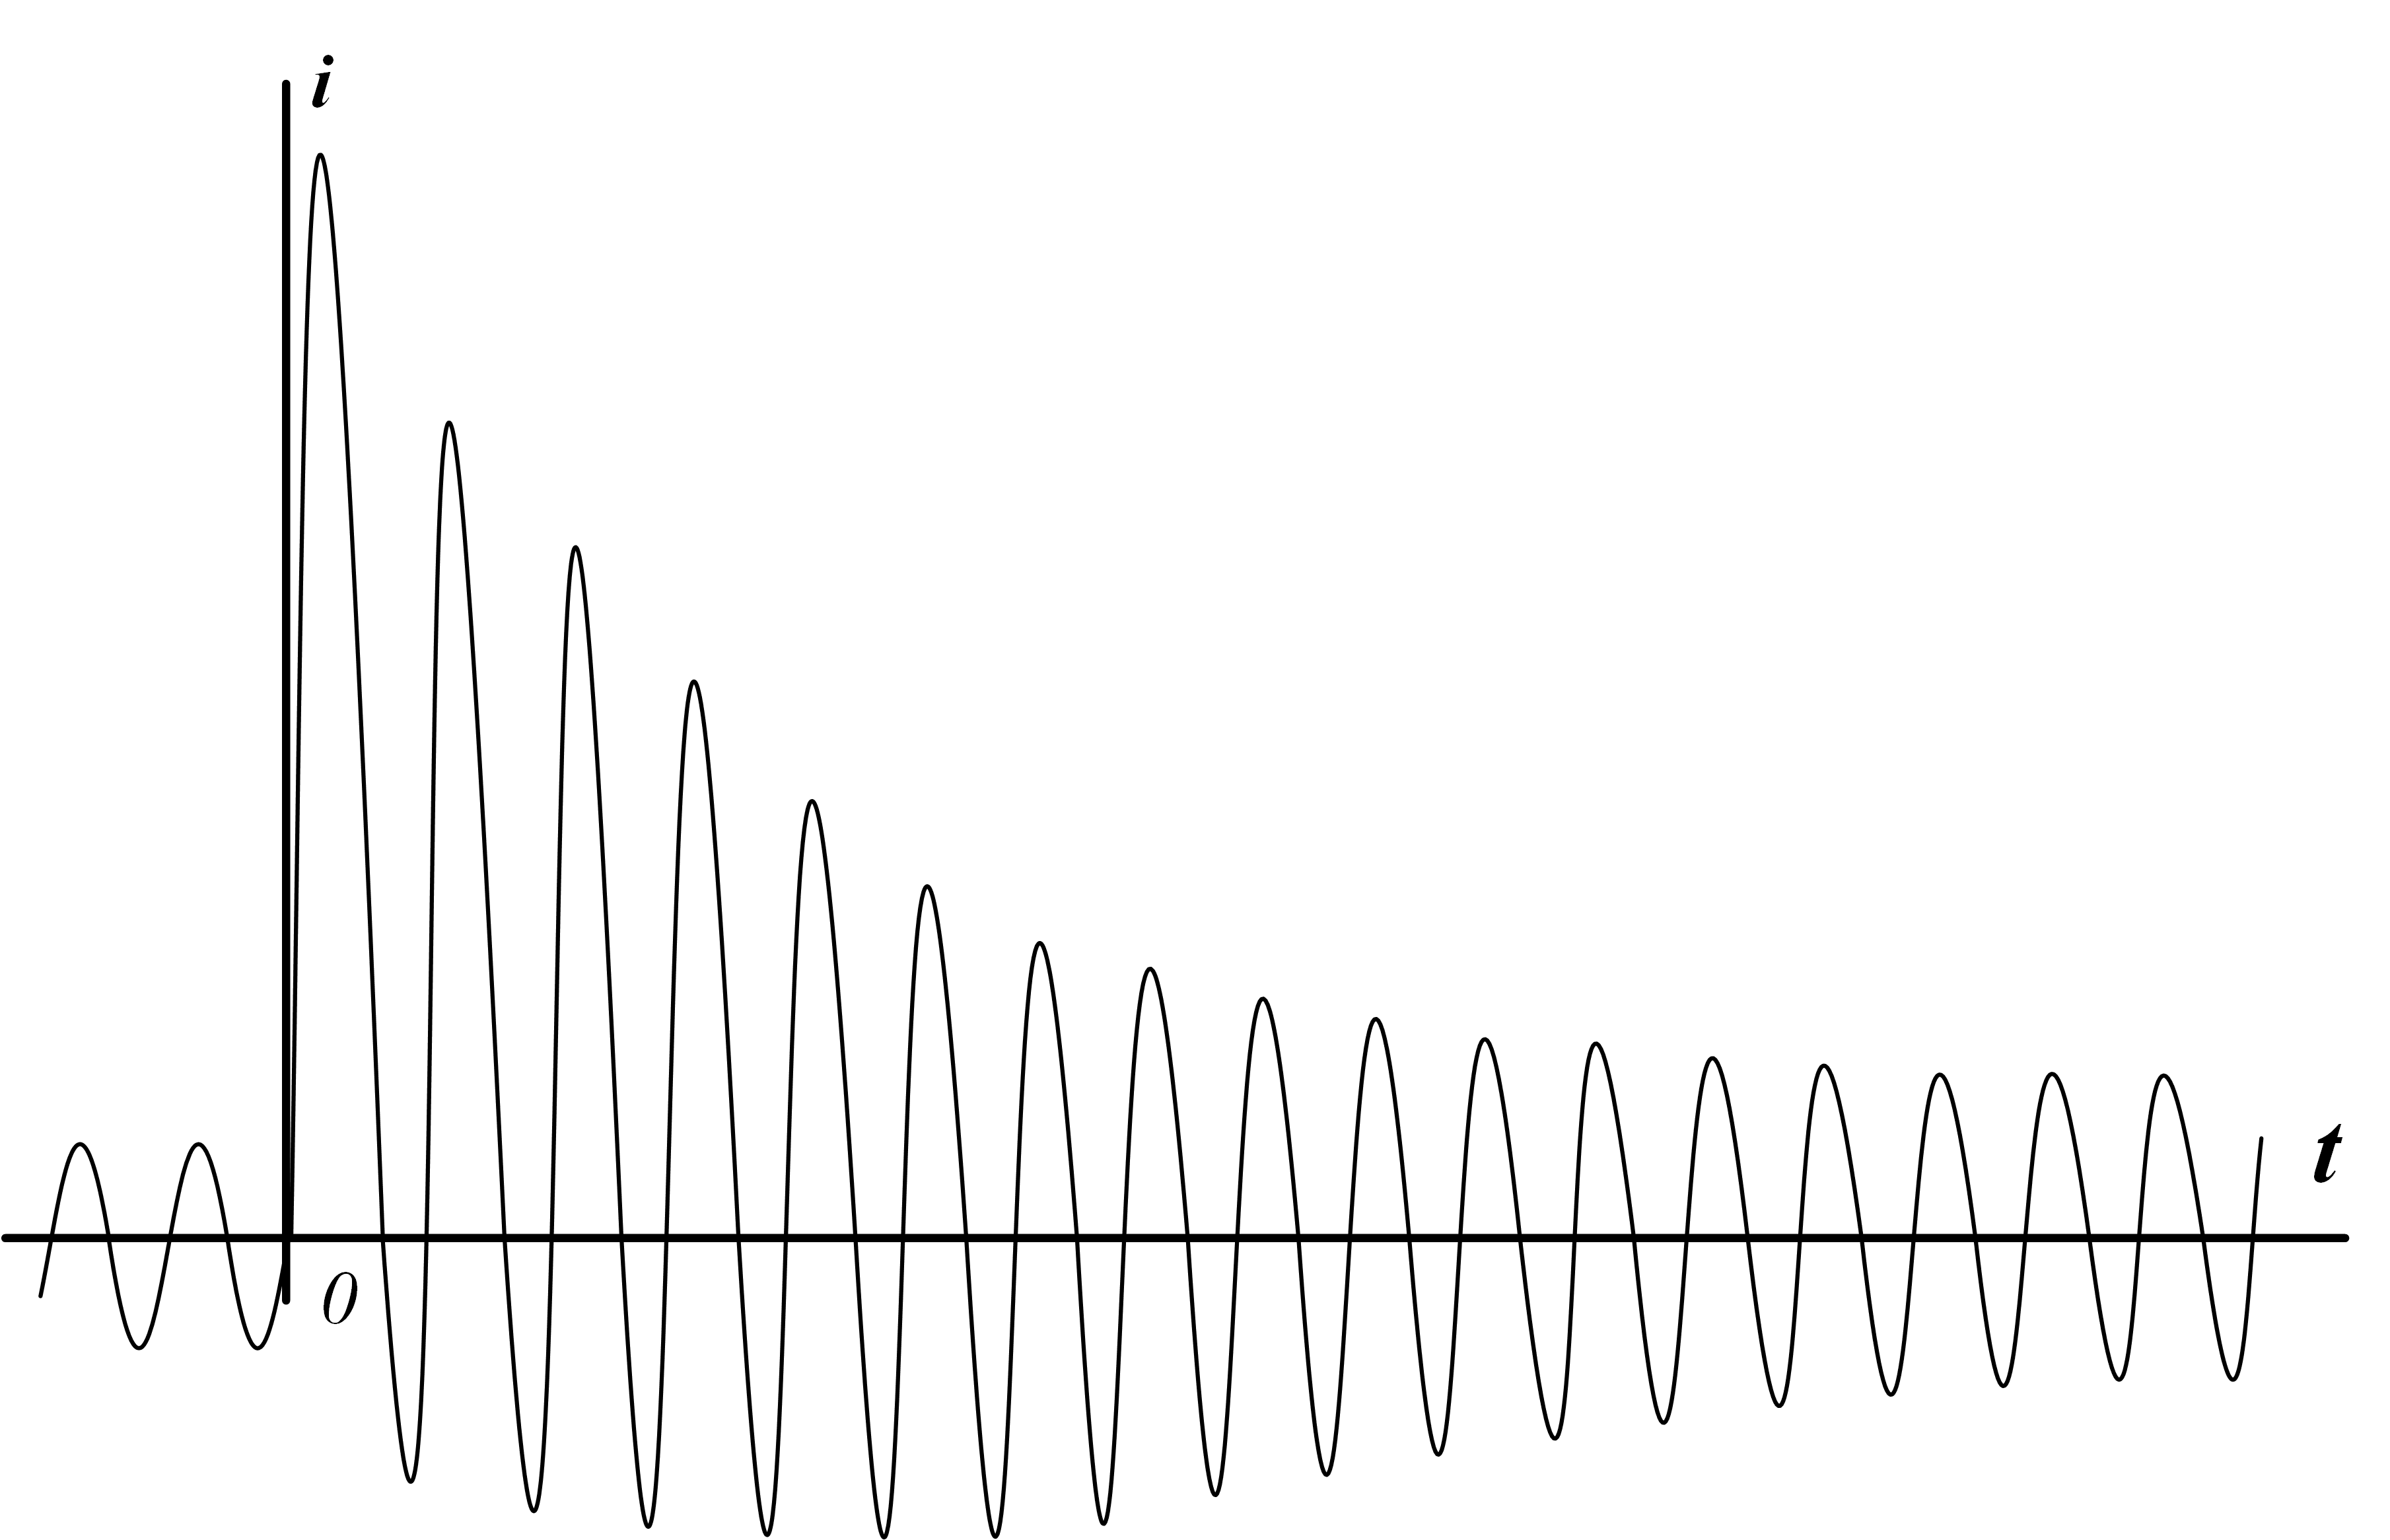
\includegraphics[width=0.7\linewidth]{pic/1-2_a} \\ \textit{а)}}
	\end{minipage}
	\vfill
	\begin{minipage}[h]{1\linewidth}
		\center{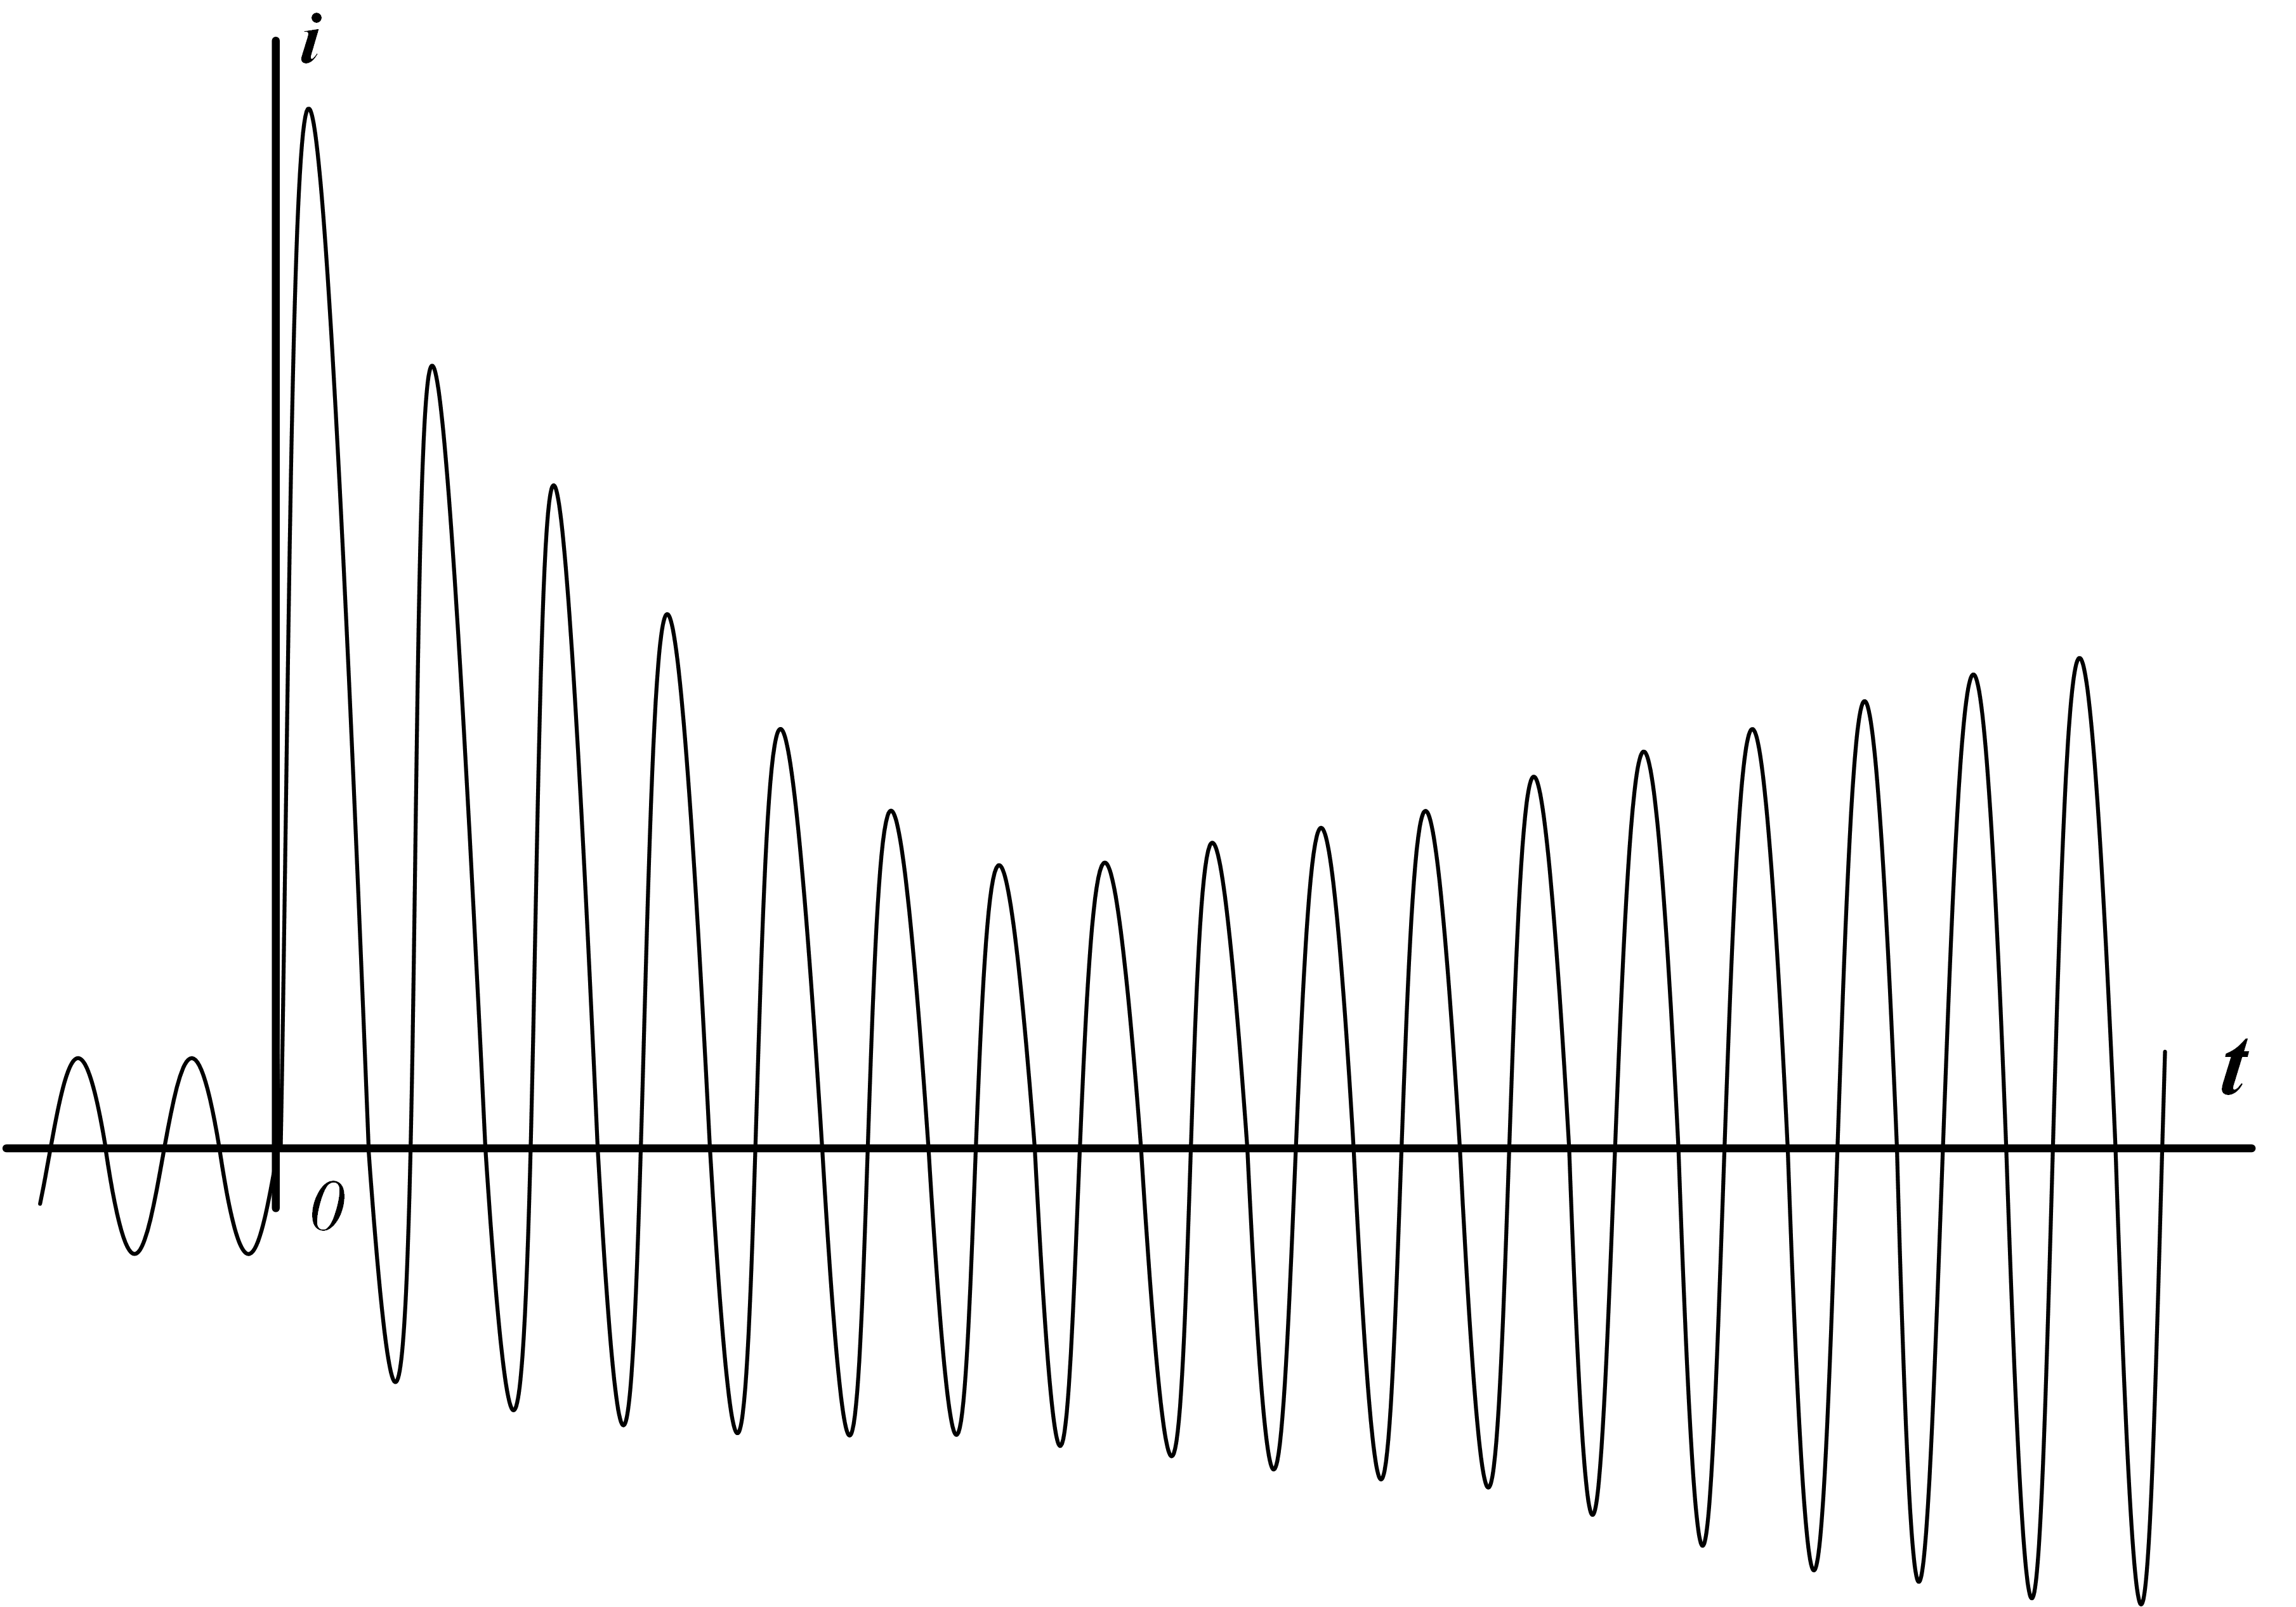
\includegraphics[width=0.7\linewidth]{pic/1-2_b} \\ \textit{б)}}
	\end{minipage}
	\caption{Осциллограммы токов при внезапном коротком замыкании. \textit{а} --- при отстутствии автоматического регулирования возбуждения; \textit{б} --- при наличии такого регулирования.}
	\label{ris:1-2 toki_kz_bez_arv_i_s_nim}
\end{figure}

Для иллюстрации процесса короткого замыкания на рис.~\ref{ris:1-2 toki_kz_bez_arv_i_s_nim} приведены типичные осциллограммы тока короткого замыкания при отсутствии автоматического регулирования возбуждения (рис.~\ref{ris:1-2 toki_kz_bez_arv_i_s_nim},а) и при наличии его (рис.~\ref{ris:1-2 toki_kz_bez_arv_i_s_nim},б). В начальной стадии обе осциллограммы практически одинаковы. Это объясняется тем, что здесь их характер определяется главным образом затуханием возникших свободных токов, а нарастание тока возбуждения от действия АРВ благодаря магнитной инерции еще очень мало. В дальнейшем, как видно, при отсутствии АРВ кривая постепенно переходит в синусоиду нового установившегося режима. При наличии АРВ амплитуда кривой тока, достигнув некоторого наименьшего значения, вновь возрастает, стремясь к установившемуся значению, которое, естественно, больше, чем при отсутствии АРВ. Возрастающий характер кривой тока при наличии АРВ обычно получается при заметной удаленности короткого замыкания относительно генератора.

Для дополнительной иллюстрации характерных переходных процессов приведем еще несколько осциллограмм. На рис. 1-3 показаны осциллограммы токов в фазе статора, обмотке возбуждения и продольной демпферной обмотке синхронного генератора мощностью 50~\textit{Мвт} при внезапном трехфазном коротком замыкании на его выводах. До короткого замыкания генератор работал на холостом ходу и его АРВ было отключено. На \colorbox{red}{рис. 1-4} приведены осциллограммы тока фазы статора асинхронного двигателя 600~\textit{квт} и потребляемой им активной мощности при трехфазном коротком замыкании вблизи двигателя и при его дальнейшем самозапуске после отключения короткого замыкания (спустя примерно 1,2~\textit{сек}).

\section{Причины возникновения и следствия}
\label{sec:1-2 prichiny_vozniknoveniia_i_sledstviia}

Основной причиной возникновения рассматриваемых в дальнейшем электромагнитных переходных процессов являются преимущественно короткие замыкания. Последние в свою очередь являются результатом нарушений изоляции электрического оборудования, которые вызываются старением изоляционных материалов, перенапряжениями, недостаточно тщательным уходом за оборудованием и непосредственными механическими повреждениями (например, повреждение кабеля при выполнении земляных работ без должной осторожности и т.~п.). В практике наблюдались случаи, когда короткие замыкания возникали от перекрытия токоведущих частей животными и птицами.

При осуществлении упрощенных схем электрических соединений понижающих подстанций, как известно, используют специальные аппараты --- короткозамыкатели (одно- и двухфазные); последние создают преднамеренные короткие замыкания с целью быстрых отключении ранее возникших повреждений.

Таким образом, наряду с короткими замыканиями случайного характера в системе имеют место также преднамеренные короткие замыкания, вызываемые действием установленных короткозамыкателей.

Социалистическое хозяйство предъявлёт особые требования к безаварийному электроснабжению всех потребителей электроэнергии. Поэтому внимание и усилия работников в области электроэнергетики должны быть направлены на соблюдение этих требований. Для этого должно быть в первую очередь обеспечено строгое соблюдение Правил технической эксплуатации электрических установок. Помимо того, требуется непрерывное повышение качества продукции, выпускаемой электротехнической промышленностью.

В зависимости от места возникновения и продолжительности повреждения его последствия могут иметь местный характер или, напротив, могут отражаться на всей системе.

Так, например, при коротком замыкании в удаленной точке сети величина тока короткого замыкания составляет лишь незначительную долю номинального тока питающих генераторов и возникновение такого короткого замыкания воспринимается ими как небольшое увеличение нагрузки. Сильное снижение напряжения получается вблизи места трехфазного короткого замыкания, в то время как в других точках системы наблюдается едва заметное снижение напряжения, причем от действия автоматического регулирования возбуждения оно быстро восстанавливается до нормального. Следовательно, при рассматриваемых условиях опасные последствия короткого замыкания проявляются лишь в ближайших к месту короткого замыкания частях системы.

Аналогичная картина, но выраженная не в столь резкой форме, наблюдается при пуске крупных двигателей, синхронных компенсаторов, при включении генераторов способом самосинхронизации, а также при их несинхронном включении.

Обрыв фазы слабо загруженной цепи, очевидно, не вызовет каких-либо существенных изменений режима в системе. Напротив, такой обрыв в цепи с большим нагрузочным током может привести к весьма существенным изменениям токов и напряжений в системе.

Ток короткого замыкания даже в тех случаях, когда он мал по сравнению с номинальным током генератора, обычно во много раз превышает номинальный ток самой самой ветви, поэтому и при кратковременном прохождении тока короткого замыкания он может вызвать дополнительный нагрев токоведущих элементов и проводников выше допустимого.

Кроме теплового действия, токи короткого замыкания вызывают между проводниками большие механические усилия, которые особенно велики в начальной стадии процесса короткого замыкания, когда ток достигает максимума. При недостаточной прочности проводников и их креплений они могут быть разрушены при коротком замыкании. Равным образом это относится к электрическим машинам и аппаратам, надежность которых может быть обеспечена при учете всех проявлений коротких замыканий.

Глубокое снижение напряжения и резкое искажение его симметрии, которое возникают при коротких замыканиях и образовании продольной несимметрии, вредно отражаются иа работе потребителей. Так, уже при понижении напряжения на 30--40\% в течение 1~\textit{сек} и более достаточно загруженные двигатели промышленного предприятия могут остановиться, что вызовет народнохозяйственный ущерб. Оставаясь включенными в сеть, остановившиеся двигатели могут вызвать дальнейшее снижение напряжения в сети, т.~е. полное нарушение нормального электроснабжения не только данного предприятия, но и за его пределами. Следует подчеркнуть, что ряд промышленных производств вообще не допускает никаких (даже кратковременных) перерывов в подаче энергии.

При замыканиях на землю возникают неуравновешенные системы токов. Они способны создавать магнитные потоки, которые достаточны, чтобы в соседних линиях связи и сигнализации навести э.~д.~с, величины которых могут быть опасны для обслуживающего персонала и аппаратуры этих линий. Заметные мешающие влияния на линии связи возникают также при продольной несимметрии в системе.

Наконец, при задержке отключения короткого замыкания сверх допустимой продолжительности может произойти нарушение устойчивости электрической системы, что является в сущности одним из наиболее опасных последствий короткого замыкания, так как отражается на работе всей системы.

\section{Назначения расчетов и требования к ним}
\label{sec:1-3 naznacheniia_raschetov_i_trebovaniia_k_nim}

При проектировании и эксплуатации электрических установок и систем для решения многих технических вопросов и задач задач требуется предварительно произвести ряд расчетов, среди которых заметное место занимают расчеты электромагнитных переходных процессов и, в частности, процессов при внезапном коротком замыкании.

Под расчетом электромагнитного переходного процесса обычно понимают вычисление токов и напряжений в рассматриваемой схеме при заданных условиях. В зависимости от назначения такого расчета находят указанные величины для заданного момента времени или находят их изменения в течение всего переходного процесса. При этом решение обычно проводится для одной или нескольких ветвей и точек схемы.

К числу задач, для практического решения которых производят такие расчеты, относятся:

\begin{enumerate} 
	\item
	сопоставление, оценка и выбор схемы электрических соединений как отдельных установок (станций, подстанций), так и системы в целом;
	\item
	выявление условий работы потребителей при аварийных режимах;
	\item
	выбор аппаратов и проводников и их проверка по условиям работы при коротких замыканиях;
	\item
	проектирование и настройка устройств релейной защиты и автоматизации;
	\item
	определение условий несинхронного включения синхронных машин и включения их способом самосинхронизации;
	\item
	конструктивные решения элементов распределительных устройств и, в частности, шинопроводов на большие рабочие токи;
	\item
	определение числа заземленных нейтралей и их размещения в системе;
	\item
	выбор числа и мощности компенсирующих дугогасящих устройств;
	\item
	определение влияния линий электропередачи на провода связи и сигнализации;
	\item
	проектирование и проверка защитных заземлений;
	\item
	подбор характеристик разрядников для защиты от перенапряжений (включая защиту конденсаторов установок продольной компенсации);
	\item
	оценка и определение параметров гашения поля синхронных машин;
	\item
	оценка и выбор систем возбуждения синхронных машин;
	\item
	проведение различных испытаний;
	\item
	анализ происшедших аварий.
\end{enumerate}

Особенностью расчетов при решении задач, встречающихся в эксплуатации, является необходимость учета конкретных условий рассматриваемого переходного процесса. Напротив, при проектировании часто довольствуются приближенными данными. Поэтому в первом случае требуется большая точность.

Так, например, благодаря тому, что интервалы между параметрами, характеризующими различные типы аппаратов в отношении их устойчивости при коротких замыканиях, достаточно большие, точность расчета для выбора таких аппаратов может быть невелика. Напротив, точность расчета для целей релейной защиты и автоматизации обычно должна быть значительно выше. Здесь, как впрочем и я ряде других случаев, часто требуется выявлять как наибольшие, так и наименьшие возможные величины токов и напряжений, сдвиг между ними в отдельных фазах или между отдельными их симметричными составляющими, их распределение в схеме и т.~п.

Неменьшие требования предъявляются к расчетам для анализа аварий, а также к расчетам, проводимым для различных исследовательских целей.

Краткие сведения о расчетных условиях даны в~§\ref{sec:2-2 poniatie o raschetnykh usloviiakh}.



















\chapter{Общие указания к выполнению расчетов}

\section{Основные допущения}

Как отмечалось выше, расчет электромагнитного переходного процесса в современной электрической системе с учетом всех имеющих место условий и факторов чрезвычайно сложен и практически невыполним. Поэтому, чтобы упростить задачу и сделать ее решение практически возможным, вводят ряд допущений. Последние зависят прежде всего от характера и постановки самой задачи. Те допущения, которые вполне пригодны при решении одной задачи, могут быть совершенно неприемлемыми при решении другой.

Каждый из практических методов расчета, электромагнитных переходных процессов, в частности процесса при коротком замыкании, основан на некоторых допущениях, касающихся преимущественно возможности использование упрощённых представлений об изменении свободных токов в сложных схемах с несколькими источниками, о разных способах учета автоматического регулирования возбуждения синхронных машин и т.~п. C ними читатель познакомится в ходе дальнейшего изложения материала. Здесь же остановимся только на тех основных допущениях, которые обычно принимают при решении большинства практических задач, связанных с определением токов и напряжений при электромагнитных переходных процессах. К  числу таких допущений следует отнести:

\begin{enumerate} 
	\item
	отсутствие насыщения магнитных систем. При этом все схемы оказываются линейными, расчет которых значительно проще; в частности, здесь могут быть использованны любые формы принципа наложения.
	\item
	Пренебрежение токами намагничивания трансформаторов и автотрансформаторов. Единственным исключением их этого допущения является случай, когда трехстержневой трансформатор с соединением обмоток $ Y_{0}/Y_{0} $ включен на напряжение нулевой последовательности (см.~\colorbox{red}{§12-5}).
	\item
	Сохранение симметрии трехфазное системы. Оня нарушается обычно лишь для какого-либо одного элемента, что происходит в результату его повреждения, или преднамеренно по специальным соображениям (см. гл.~\colorbox{red}{15}).
	\item
	Пренебрежение емкостными проводимостями. Это допущение обычно является, уместным и заметно не искажает результаты решения, если в рассматриваемой схеме нет продольной компенсации индуктивности цепи, а также дальних линий передач напряжением выше 220~\textit{кв}. При рассмотрении простых замыканий на землю (см.~§\colorbox{red}{17-2}) это допущение, разумеется, совсем непригодно, так как в данном случае ток замыкается именно через емкостные проводимости.
	\item
	Приближенный учет нагрузок. В зависимости от стадии переходного процесса нагрузку приближенно характеризуют некоторым постоянным сопротивлением, обычно чисто индуктивным (см.~\colorbox{red}{§5-4 и §6-5}).
	\item
	Отсутствие активных сопротивлений. Это допущение в известной мере условно. Оно приемлемо при определении начальных и конечных значений отдельных величин, характеризующих переходный процесс в основных звеньях высокого напряжения электрической системы; при этом приближенный учет активных сопротивлений находит отражение при оценке постоянных времени затухания свободных составляющих рассматриваемых величин. В тех же случаях, когда подобный расчет проводится для протяженной кабельной или воздушной сети с относительно небольшими сечениями проводников (особенно линии со стальными проводами), а также для для установок и сетей напряжением до 1~\textit{кв}, данное допущение непригодно (см.~\colorbox{red}{гл. 17}).
	\item
	Отсутствие качаний синхронных машин. Если задача ограничена рассмотрением лишь начальной стадии переходного процесса (т.~е. в пределах 0,1--0,2~\textit{сек} с момента нарушения режима до отключения повреждения), это допущение обычно не вносит заметной погрешности (особенно в токе в месте повреждения). Однако при возникновении существенных качаний или выпадении машин из синхронизма достаточно надежный результат может быть получен лишь с учетом (хотя бы приближенным) такого процесса (см.~\colorbox{red}{гл. 19}).
\end{enumerate}

\section{Понятие о расчетных условиях}

В соответствии с целевым назначением проводимого на практике расчета электромагнитного переходного процесса устанавливают исходные расчетные условия. Они весьма разнообразны и при решении разных задач могут быть даже противоположными.

Так, например, для выбора выключателя по условиям его работы при коротком замыкании должны быть определены соответствующие возможные наибольшие величины тока короткого замыкания. С этой целью исходят из предположения, что короткое замыкание происходит в то время, когда включено наибольшее число генераторов, что вид короткого замыкания такой, при котором ток достигает наибольшей величины, что короткое замыкание металлическое и что оно произошло непосредственно у выводов самого выключателя. Помимо того, здесь устанавливают расчетное время размыкания контактов выключателя и цикл производимых им операций (включение и отключение).

Для выбора трубчатого разрядника требуется знать не только наибольшую, но и возможную наименьшую величину тока короткого замыкания, для определения которой, разумеется, должны быть приняты совсем иные расчетные условия.

Большое разнообразие расчетных условий встречается при выполнении расчетов для выбора и настройки устройств релейной защиты и автоматики. В них устанавливаются исходные предшествующие режимы заданной системы, число и расположение заземленных нейтралей, виды повреждений, и последовательность отключения поврежденного участка и т.~п.

При решении вопроса гашения поля синхронной машины в качестве расчетного режима может быть как режим короткого замыкания, так и холостого хода.

Приведенные примеры показывают, сколь велико разнообразие расчетных условий. Обоснование расчетных условий для конкретных технических задач (с учетом вероятности отдельных факторов) является одним из важных вопросов соответствующих специальных дисциплин.

\section{Система относительных единиц}

Представление любых физических величин не в обычных для них соответствующих именованных единицах, а в относительных, безразмерных единицах позволяет существенно упростить некоторые теоретические выкладки и придать им более общий характер. Равным образом и в практических расчетах такое представление величин придает результатам большую наглядность и позволяет быстрее ориентироваться в порядке определяемых значений. Благодаря этому система относительных единиц широко используется, хотя на первый взгляд она может казаться несколько искусственной и даже излишней.

С выражением величин в относительных единицах (в долях или процентах) читатель уже встречался при изучении электрических машин, где реактивности обычно выражают в долях единицы, напряжения короткого замыкания трансформаторов --- в процентах, пусковые токи и моменты асинхронных двигателей --- в кратностях от их номинальных значений и т.~д. Теперь нам нужно познакомиться с системой относительных единиц в более широком аспекте, имея в виду использование ее при решении различных вопросов и задач для схем с произвольным числом всевозможных элементов.

Напомним, что под относительным значением какой-либо величины следует понимать ее отношение к другой одноименной величине, выбранной за единицу измерения. Следовательно, чтобы выразить отдельные величины в относительных единицах, нужно прежде всего выбрать те величины, которые должны служить соответственными единицами измерения, или, как говорят, установить базисные единицы (или условия).

Пусть за базисный ток и базисное междуфазное напряжение приняты некоторые произвольные величины $ I_{\mbox{б}} $ и $ U_{\mbox{б}} $. Тогда базисная мощность трехфазной системы, очевидно, будет:

\begin{equation}
	\label{eq:chap2 S_baz}
	S_{\mbox{б}} = \sqrt{3}U_{\mbox{б}}I_{\mbox{б}}
\end{equation}

и базисное сопротивление

\begin{equation}
	\label{eq:chap2 z_baz}
	z_{\mbox{б}} = \frac{U_{\mbox{б}}}{\sqrt{3}I_{\mbox{б}}}
\end{equation}

т.~е. оно подчинено закону Ома, чтобы обеспечить тождественную запись этого закона как в именованных, так и в относительных единицах.

Как видно, из четырех базисных единиц $ I_{\mbox{б}} $, $ U_{\mbox{б}} $, $ S_{\mbox{б}} $ и $ z_{\mbox{б}} $ только две могут быть выбраны произвольно, а две другие уже получаются из указанных соотношений. Фазные и междуфазные базисные напряжения, а также фазные и линейные базисные токи связаны между собой известными соотношениями для симметричной трехфазной системы. Следует особо подчеркнуть, что выбранные базисные единицы служат для, измерения как полных величин, так и их составляющих (активных, реактивных и~пр.).

% 29 страница









%TODO: Раздел второй - ЭЛЕКТРОМАГНИТНЫЕ ПЕРЕХОДНЫЕ ПРОЦЕССЫ ПРИ СОХРАНЕНИИ СИММЕТРИИ ТРЕХФАЗНОЙ ЦЕПИ
\chapter{Переходный процесс в простейших трехфазных цепях}
\label{chap:3 perehodnyi_protcess_v_prosteishikh_trekhfaznykh_tcepiakh}

\section{Постановка задачи и ее ограничения}
\label{sec:3-1 postanovka_zadachi_i_ee_ogranicheniia}

Симметричную трехфазную цепь с сосредоточенными активными сопротивлениями и индуктивностями при отсутствии в ней трансформаторных связей условимся называть \so{простейшей} трехфазной цепью.

Электромагнитный переходный процесс в такой цепи рассмотрим сначала при условии, что ее питание осуществляется от источника, сопротивление которого равно нулю и его напряжение, изменяясь с постоянной частотой, имеет неизменную амплитуду\footnote{Применение чувствительного и быстродействующего автоматического регулировании возбуждения генераторов дополнительно способствует принятию указанного предположения.}. Обычно его называют источником бесконечной  мощности.

Включение в схему такого источника, вообще говоря, соответствует теоретическому пределу, когда изменение внешних условий не влияет на работу самого источнику. Практически это имеет место, например, при коротких замыканиях в относительно маломощных электрических установках или протяженных сетях, питаемых от крупных энергетических систем (см.~\colorbox{red}{гл. 17}).

С исследованием переходных процессов в подобных условиях читатель знаком из курса теоретических основ электротехники. Поэтому задачей данной главы является кратко напомнить основные выводы такого исследования, отметить особенности многофазной цепи по сравнению с однофазной, привести некоторые упрощенные приемы расчета и обратить внимание на влияние ряда факторов.

\section{Трехфазное короткое замыкание в неразветвленной цепи}
\label{sec:3-2 trekhfaznoe_korotkoe_zamykanie_v_nerazvetvlennoi_tcepi}

Обратимся к рис.~\ref{ris:3-1 simple_3_phase_circut}, на котором представлена простейшая симметричная трехфазная цепь. В ней условно принято, что на одном ее участке имеется взаимоиндукция между фазами, а на другом она отсутствует. Цепь присоединена к источнику синусоидального напряжения с неизменными амплитудой и частотой.

Рассмотрим переходный процесс, вызванный включением выключателя \textit{B}, за которым сделана закоротка, что равносильно возникновению металлического трехфазного короткого замыкания между двумя участками данной цепи.

\begin{figure}[h]
	\center{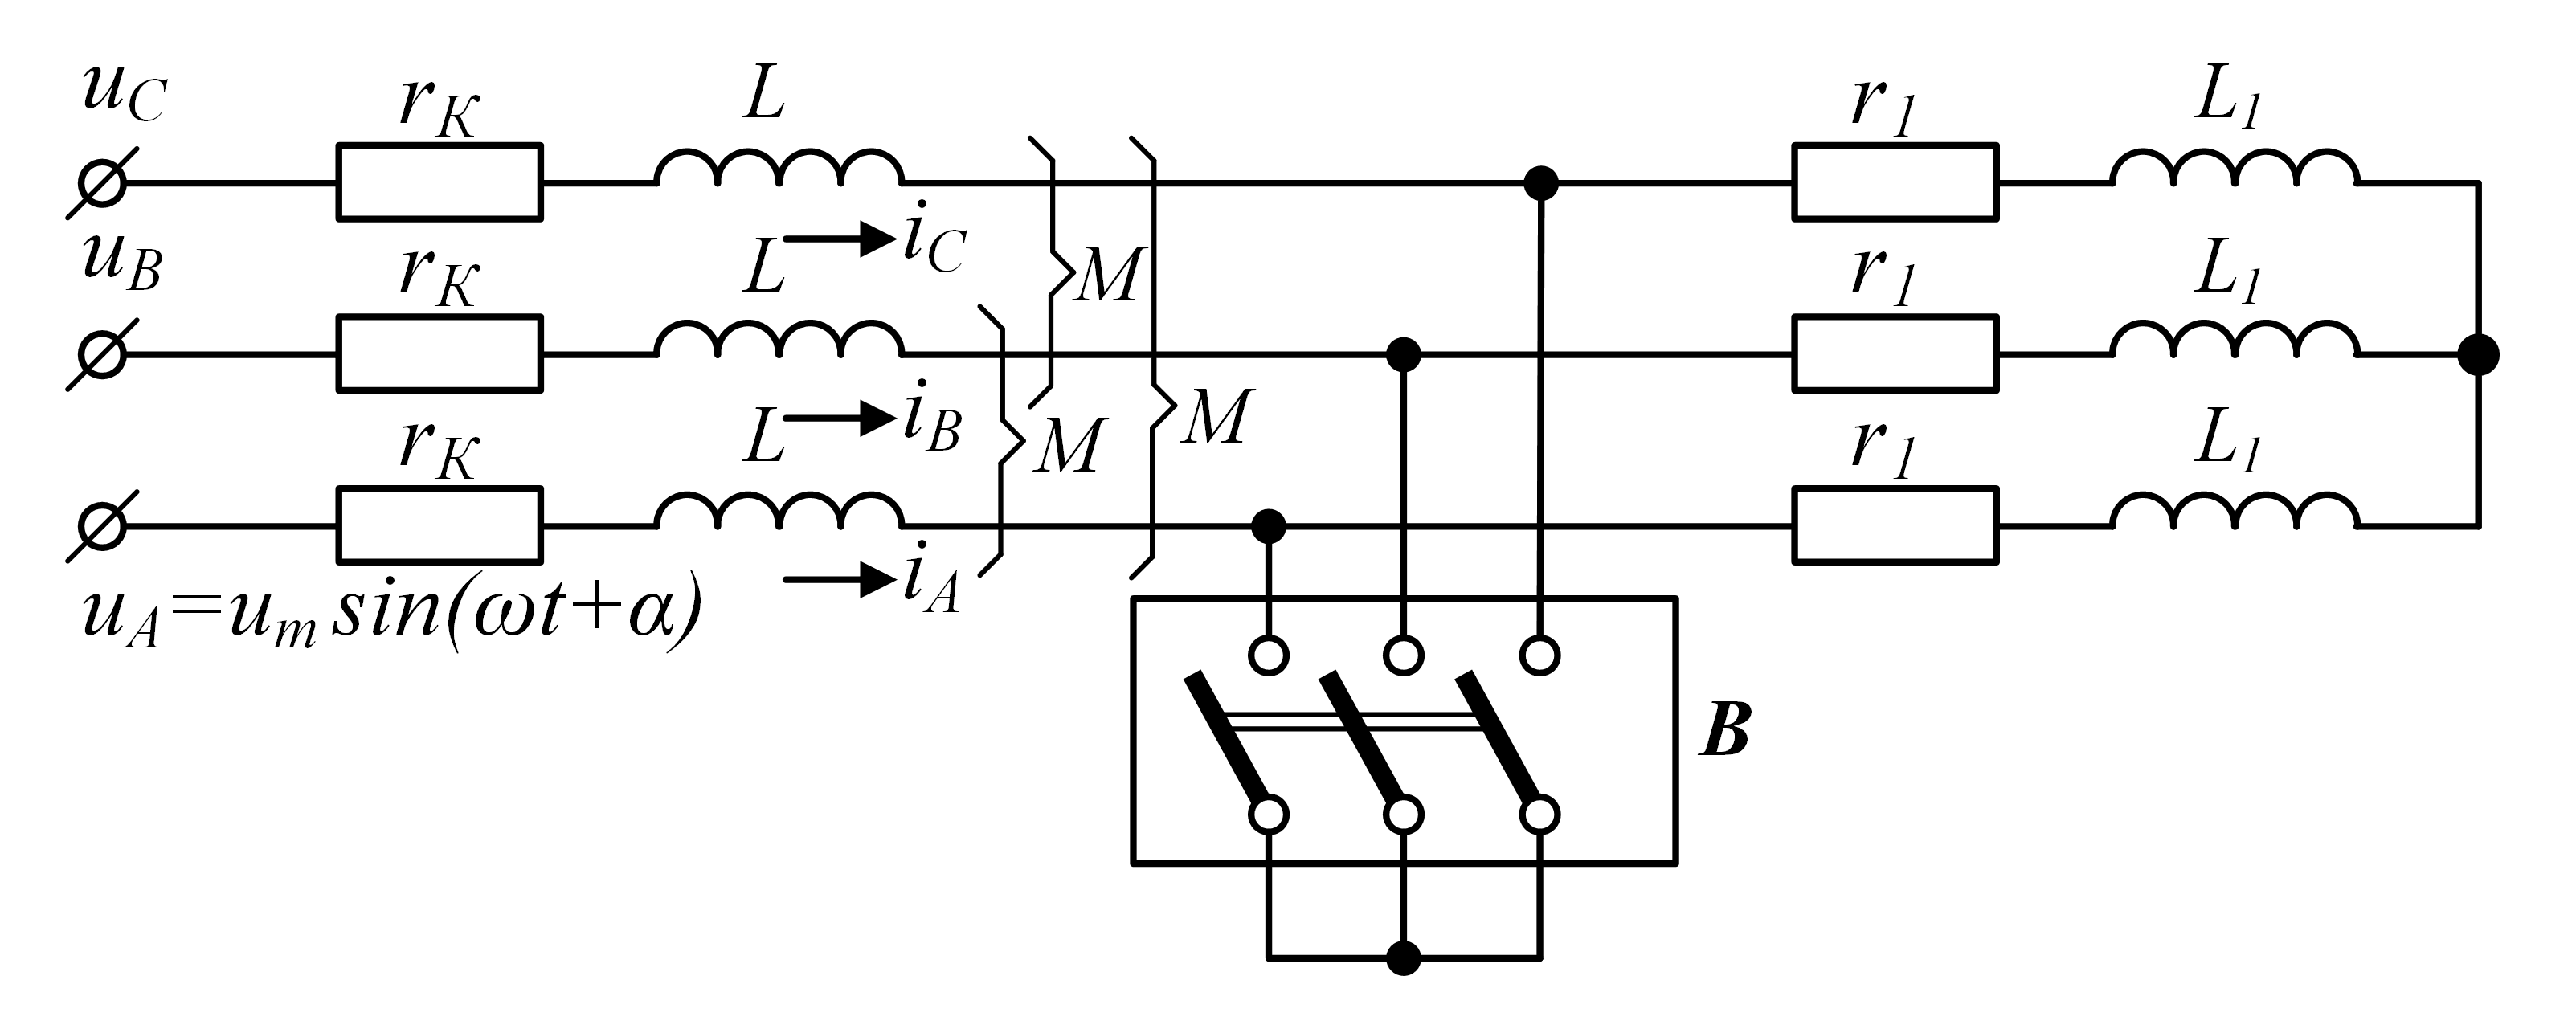
\includegraphics[width=0.9\linewidth]{pic/3-1}}
	\caption{Простейшая трехфазная электрическая цепь.}
	\label{ris:3-1 simple_3_phase_circut}
\end{figure}

Пусть векторы $ \overset{\;.}{U}_A $, $ \overset{\;.}{U}_B $, $ \overset{\;.}{U}_C $, $ \overset{\;.}{I}_A $, $ \overset{\;.}{U}_B $, $ \overset{\;.}{U}_C $ (рис.~\ref{ris:3-2 diagram})
характеризуют предшествующий режим рассматриваемой цепи, а вертикаль \textit{tt} является неподвижной линией времени, т.~е. мгновенные значения отдельных величии определяются проекциями на эту линию соответствующих вращающихся векторов. Момент возникновения короткого замыкания будем фиксировать значением угла $ \alpha $ (т.~е. \so{фазой включения}) между вектором напряжения фазы \textit{A} и горизонталью. (рис.~\ref{ris:3-2 diagram}.

После включения выключателя \textit{В} цепь рис.~\ref{ris:3-1 simple_3_phase_circut} распадается на два независимых друг от друга участка. Участок с $ r_1 $ и $ L_1 $ оказывается зашунтированным коротким замыканием и ток в нем будет поддерживаться лишь до тех пор, пока запасенная в индуктивности $ L_1 $ энергия магнитного потока не перейдет в тепло, поглощаемое активным сопротивлением $ r_1 $.

Дифференциальное уравнение равновесия в каждой фазе этого участка имеет вид:

\begin{equation}
	0 = ir_1 + L_1 \frac{di}{dt}.
	\label{eq:3-1 diff_ur}
\end{equation}

Его решение общеизвестно:

\begin{equation}
	i = i_0 e^{-t / T_{\text{а}1}}; %TODO: Проверить формулу, какая-то черка в степени
	\label{eq:3-2 diff_solve}
\end{equation}

оно показывает, что здесь имеется лишь свободный ток, который затухает по экспоненте с постоянной времени

\begin{equation}
	T_{\text{а}1} = \frac{L_1}{r_1} = \frac{x_1}{\omega r_1}, \textit{~сек}.
	\label{eq:3-3 T_a1}
\end{equation}

Начальное значение свободного тока в каждой фазе зашунтированного участка цепи, очевидно, равно предшествовавшему мгновенному значению тока, поскольку в цепи с индуктивностью не может произойти внезапного (скачком) изменения тока. В общем случае свободные токи в фазах различны, хотя их затухание, разумеется, происходит с одной и той же постоянной времени. В одной из фаз свободный ток может вообще отсутствовать, если в момент возникновения короткого замыкания предшествовавший ток в этой фазе проходил через нуль; при этом свободные токи в двух других фазах будут одинаковы по величине, но противоположны по направлению.

На рис.\colorbox{red}{3-3} слева приведены кривые изменения фазных токов в зашунтированном участке рассматриваемой цени, с учетам, что короткое замыкание произошло в момент, отвечающий положению векторов на рис.~\ref{ris:3-2 diagram}.

\begin{floatingfigure}[lflt]{0.45\linewidth}
	\centering
	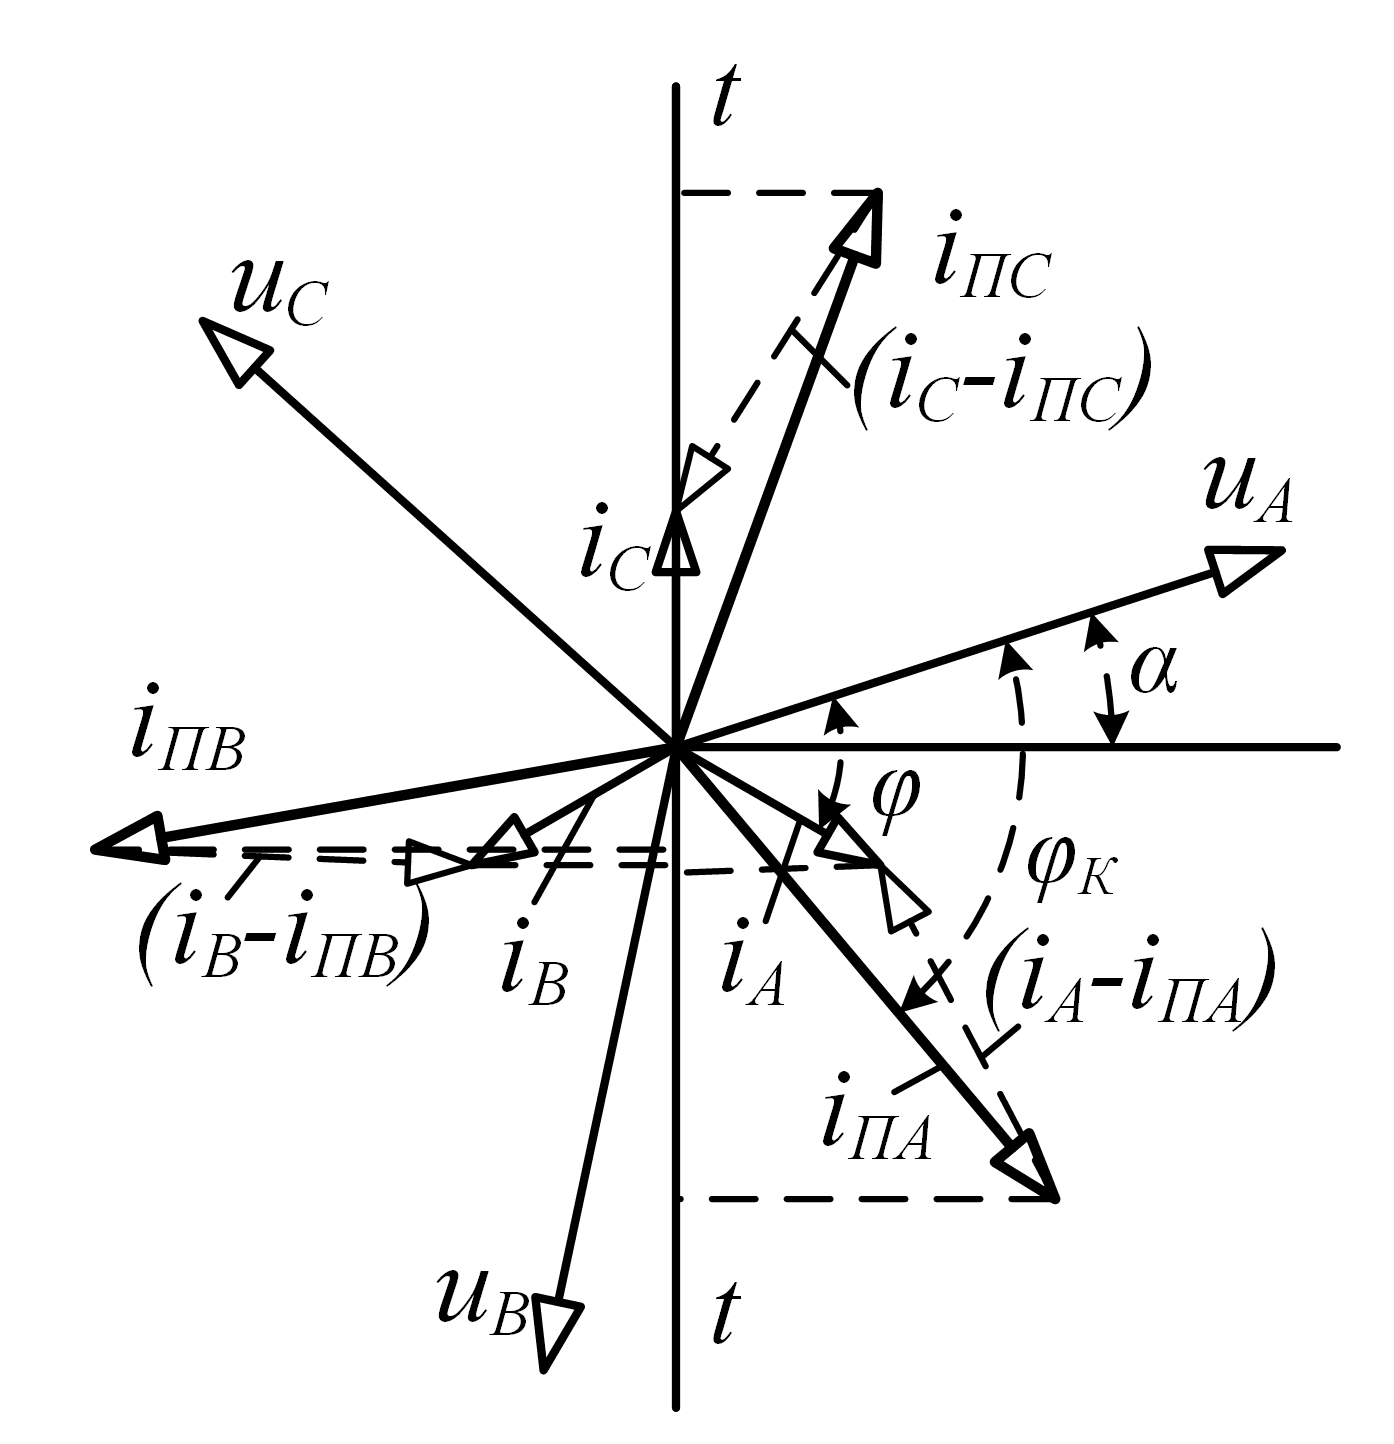
\includegraphics[width=0.40\linewidth]{pic/3-2}
	\caption{Векторная диаграмма для начального момента трехфазного короткого замыкания.}
	\label{ris:3-2 diagram}
\end{floatingfigure}

\begin{small}
	Напомним, что подкасательная в любой точке экспоненты\footnote{Обычно используют начальную часть экспоненты, где скорость изменения соответствующей величины больше и поэтому можно точнее провести касательную.} в принятом для оси времени масштабе дает значение постоянной времени, с которой происходит изменение экспоненты (рис. \colorbox{red}{3-3}). Имея в виду, что при $ t = T_{\text{а}} $ значение $ e^{-1} = 0,368 $, постоянную $ T_{\text{а}} $ обычно трактуют как время, в течение которого переменная величина снижается до 0,368 своего начального значения; при этом за начальную может быть принята любая точка кривой.
	
\end{small}

%TODO: Рисунок оказывается перед 3-2 ??!!
\begin{figure}
	\center{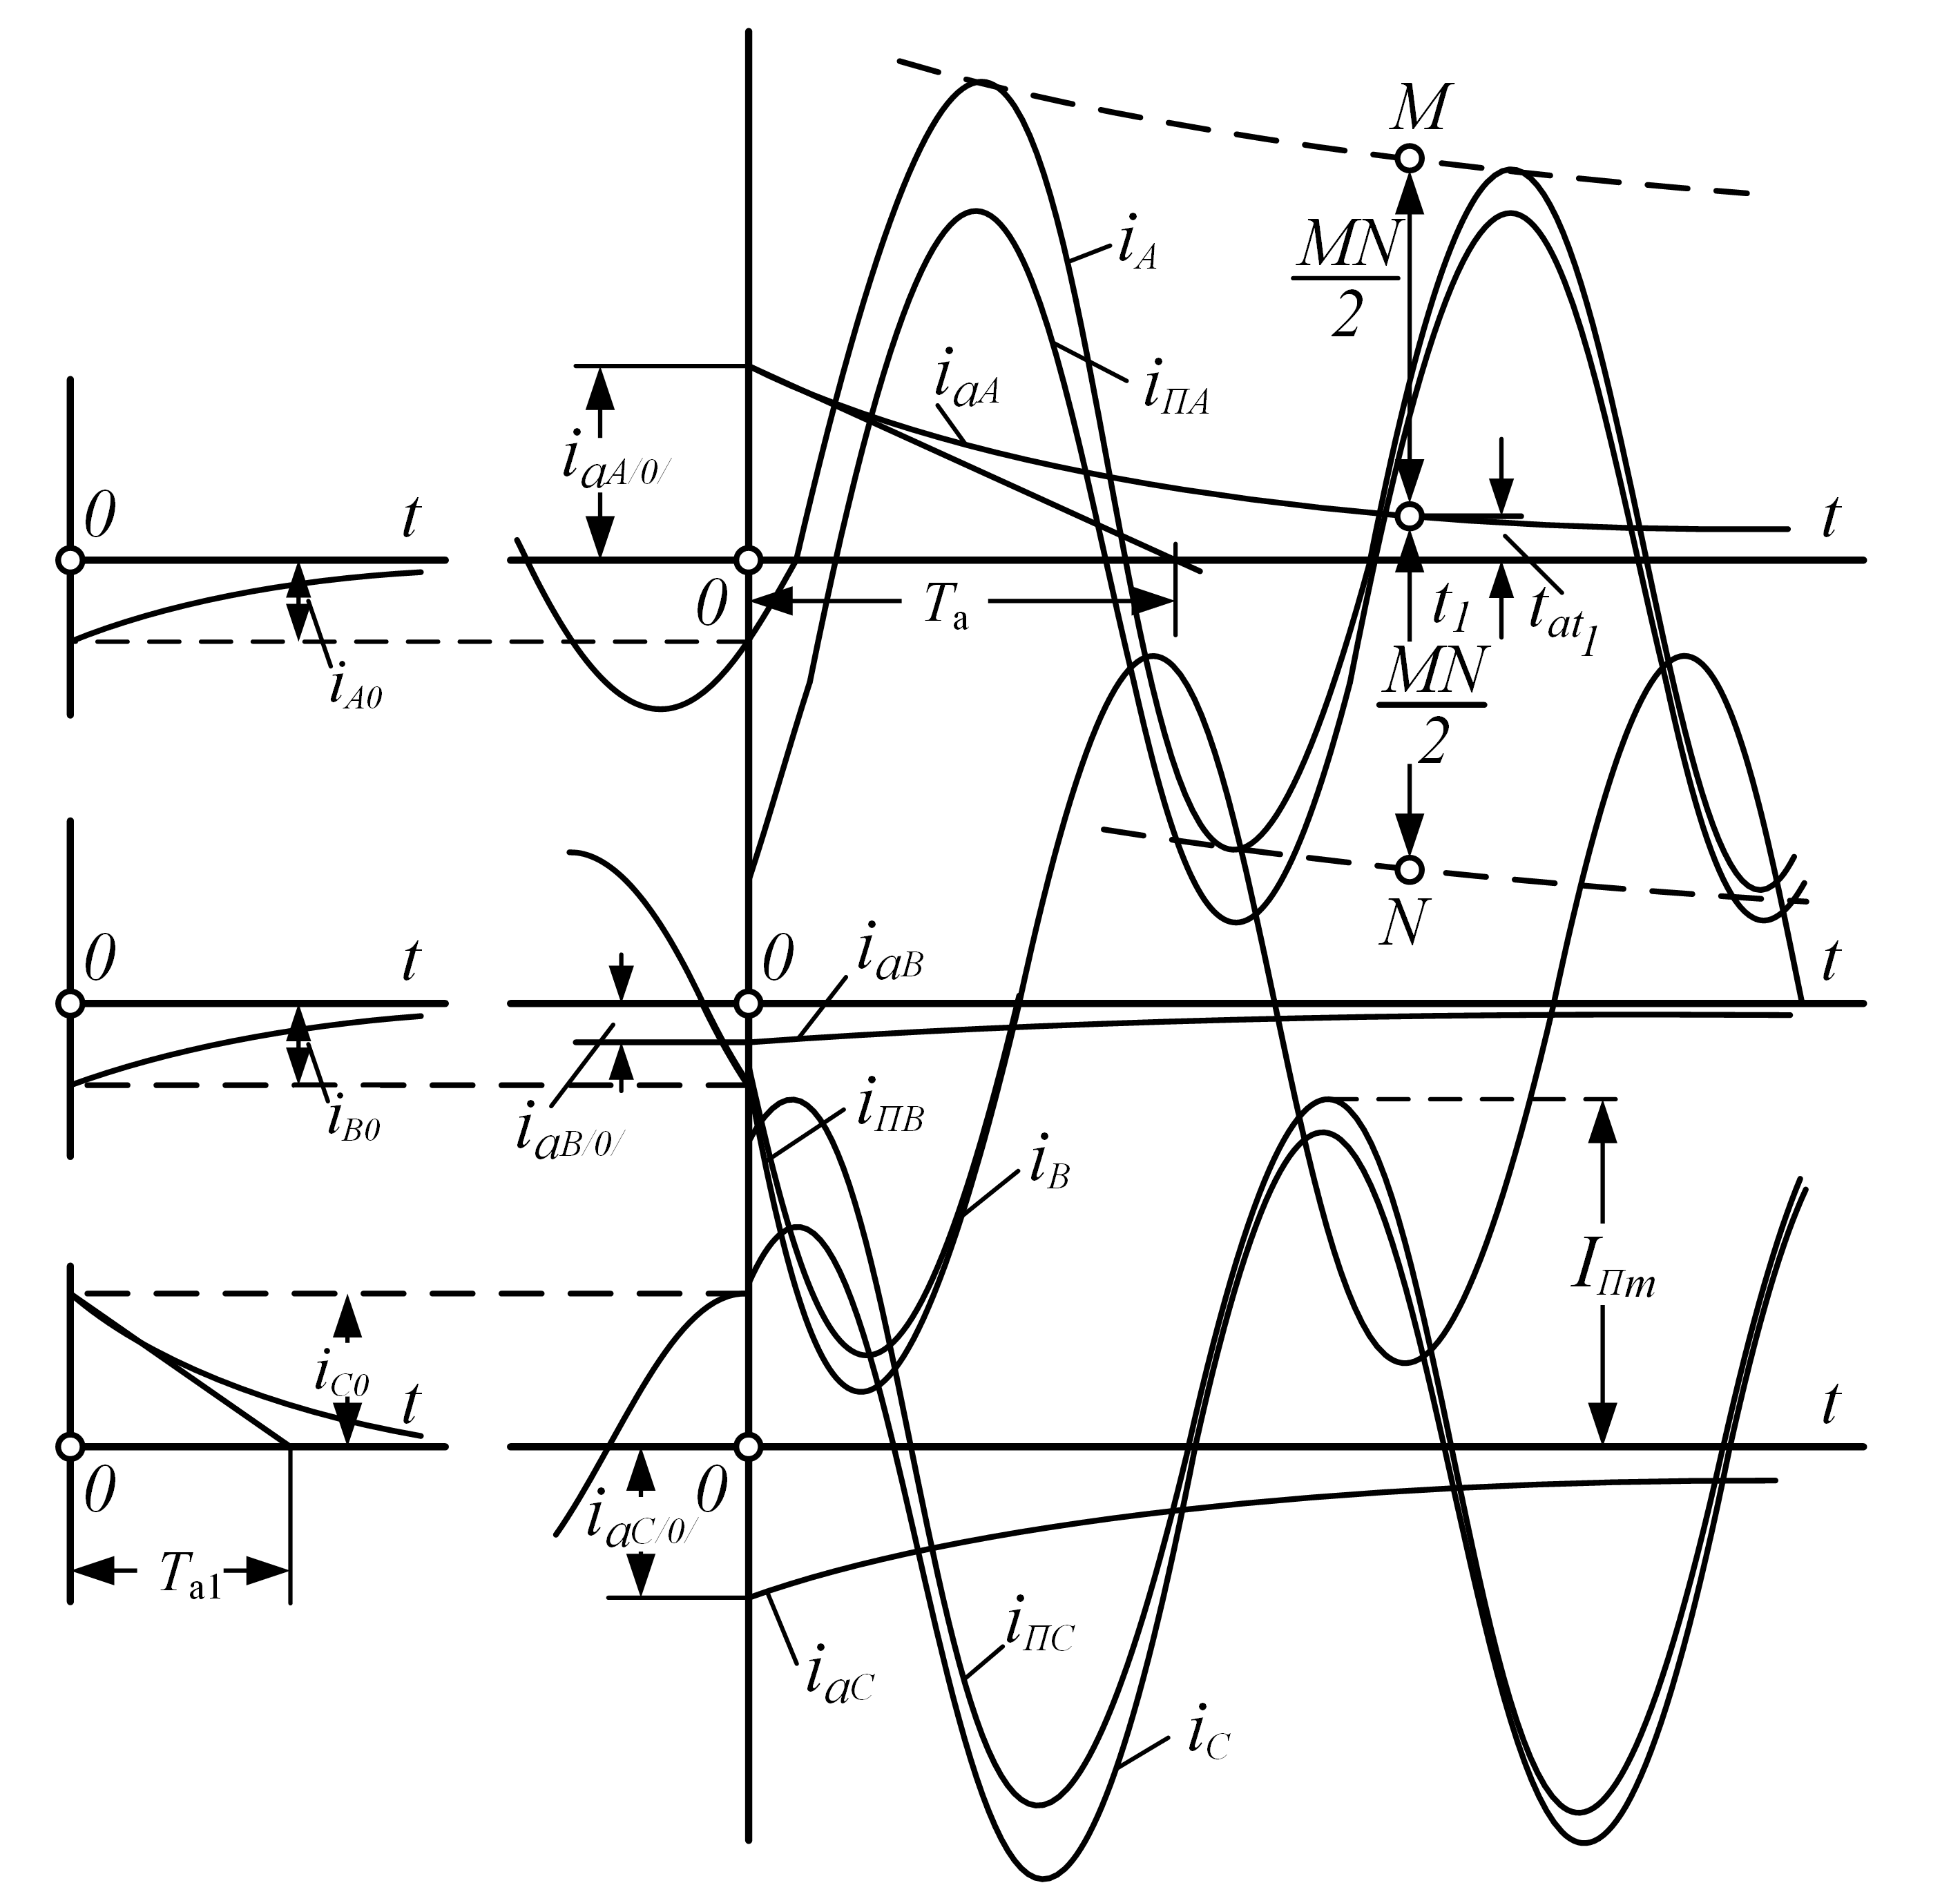
\includegraphics[width=0.85\linewidth]{pic/3-3}}
	\caption{Осциллограммы токов в фазах при внезапном трехфазном коротком замыкании в простейшей электрической цепи.}
	\label{ris:3-3}
\end{figure}

Перейдем теперь к участку цепи, который остался присоединенным к источнику. Здесь помимо свободного тока будет новый принужденный ток, величина которого, очевидно, больше предыдущего и сдвиг по фазе которого в общем случае иной. Допустим, что векторы $ I_{\text{П}A} $, $ I_{\text{П}B} $, $ I_{\text{П}C} $ (рис.~\ref{ris:3-2 diagram}) отвечают новому установившемуся режиму данного участка цепи.

Дифференциальное уравнение равновесия для любом фазы, например фазы \textit{А}, этого участка

\begin{equation*}
	u_A = i_A r_{\text{К}} + L \frac{di_A}{dt} + M \frac{di_B}{dt} + M \frac{di_C}{dt},
\end{equation*}

имея ввиду, что $ (i_B + i_C) = -i_A $, можно представить (опуская индекс фазы) как

\begin{equation}	
	u = i r_{\text{К}} + L_{\text{К}} \frac{di}{dt},
	\tag{\ref*{eq:3-1 diff_ur}а}
	\label{eq:3-1a u}
\end{equation}

где $ L_{\text{К}} = (L - M) $ --- результирующая индуктивность фазы, т.~е. индуктивность с учетом влияния двух других фаз.

Решение (\ref{eq:3-1a u}) имеет вид:

\begin{equation}	
	i = \frac{U_m}{z_{\text{К}}} sin(\omega t + \alpha - \varphi_{\text{К}}) + i_{\text{а} | 0 |} e^{-t / T_{\text{а}}}
	\tag{\ref*{eq:3-2 diff_solve}а}
	\label{eq:3-2a i}
\end{equation}

где $ z_{\text{К}} $ --- полное сопротивление присоединенного к источнику участка цепи или. короче, цепи короткого замыкания;

$ \varphi_{\text{К}} $ --- угол сдвига тока в этой цепи;
	
$ T_{\text{a}} $ --- постоянная времени цепи короткого замыкания, определяемая по (\ref{eq:3-3 T_a1}), где вместо $ L_1 $, $ x_1 $, $ r_1 $ следует ввести $ L_{\text{К}} $, $ x_{\text{К}} $, $ r_{\text{К}} $.

Первый член правой части (\ref{eq:3-2a i}) представляет периодическую слагающую тока, которая при рассматриваемых условиях является принужденным током с постоянной амплитудой $ I_{\text{П}m} = U_m / z_{\text{К}} $. Соответственно второй член представляет, как и раньше, затухающий по экспоненте свободный ток; его называют также апериодической слагающей тока. Начальное значение этой слагающей определяется из начальных условий, т.~е.

% В этом месте в книге опечатка, формула названа 3-3, нумерация дальше отличается
\begin{equation}
	i_0 = i_{\text{п}~/0/} + i_{\text{а}~/0/},
	\label{eq:3-4 i_0}
\end{equation}

откуда после подстановки соответствующих выражений имеем:

\begin{equation}
	i_{\text{а}|0|} = I_m sin(\alpha - \varphi) - I_{\text{П}m} sin(\alpha - \varphi_{\text{К}}).
	\label{eq:3-5 i_a0}
\end{equation}

Поскольку токи $ i_{\text{П}} $, $ i_0 $ являются проекциями векторов $ \overset{\;.}{I}_{\text{П}m} $ и $ \overset{\;.}{I}_m $ на линию времени, то ток $ 	i_{\text{а}|0|} $ также можно рассматривать как проекцию вектора $ (\overset{\;.}{I}_m - \overset{\;.}{I}_{\text{П}m} $ на ту же линию (рис.~\ref{ris:3-2 diagram}). В зависимости от фазы включения $ \alpha $ начальное значение тока $ 	i_{\text{а}|0|} $ может изменяться от возможной наибольшей величины, когда вектор $ (\overset{\;.}{I}_m - \overset{\;.}{I}_{\text{П}m} $ параллелен линии времени, до нуля, когда этот вектор нормален к ней. В трехфазной системе такие частные условия, разумеется, могут быть лишь в одной из фаз.

%TODO: Рисунок 3-4

На рис. \colorbox{red}{3-3} справа представлены кривые изменения токов в фазах рассматриваемого участка при трехфазном коротком замыкании. Как видно, чем больше апериодическая слагающая тока, тем больше смещение кривой полного тока относительно оси времени. Эту слагающую можно рассматривать как криволинейную ось симметрии кривой полного тока, из которой ее легко выделить. Для этого нужно сначала провести огибающие по максимальным положительным и отрицательным значениям заданной кривой тока (см. пунктирные линии у кривой тока фазы \textit{А} на \colorbox{red}{рис. 3-3}). Каждая точка кривой апериодической слагающей лежит посредине вертикального отрезка между этими огибающими.

Из (\colorbox{red}{3-4}) и рис. \colorbox{red}{3-2} следует, что наибольшее значение апериодической слагающей тока определяется не только фазой включения, но также предшествующим режимом цепи. Так, например, при отсутствии предшествующего тока в данной цепи величина 
при отсутствии величина $ i_{\text{а}/0/} $ может достигать амплитуды периодической слагающей, если в момент короткого замыкания эта слагающая проходит через свой положительный или отрицательный максимум (рис.\colorbox{red}{3-4}). Обычно этот случай рассматривается как расчетный\footnote{Хотя возможны частные случаи, когда начальное значение апериодической слагающей тока превышает амплитуду периодической слагающей.}.

Важно отметить, что фаза включения, при которой возникает наибольшее значение апериодической слагающей, еще не предопределяет того, что именно при ней будет максимум мгновенного значения полного тока. В самом деле, из (\ref{eq:3-2a i}) и (\ref{eq:3-5 i_a0}) при отсутствии предшествующего тока ($ I_m = 0 $) следует, что полный ток в цепи короткого замыкания является функцией двух независимых переменных: времени $ t $ и фазы включения $ \alpha $ и выражается уравнением









\chapter{Переходный процесс в неподвижных магнитосвязанных цепях}
\label{chap:4 perehodnyi_protcess_v_nepodvizhnykh_magnitosviazannykh_tcepiakh}

\section{Общие замечания}
\label{sec:4-1 obshchie_zamechaniia}

Протекание электромагнитного переходного процесса в магнитносвязанных цепях имеет некоторые характерные особенности. Рекомендуется обратить особое внимание на основные закономерности и соотношения, рассматриваемые в настоящей главе; они в значительной мере облегчат понимание более сложных явлений, которые исследуются в дальнейшем применительно к вращающимся электрическим машинам.

В качестве основной предпосылки в соответствии с ранее принятыми допущениями считаем, что между токами и напряжениями рассматриваемых цепей сохраняется линейная зависимость и, следовательно, они могут быть связаны линейными дифференциальными уравнениями с постоянными коэффициентами. Для силовых трансформаторов и автотрансформаторов в условиях короткого замыкания (или значительных перегрузок) это допущение практически выполняется, поскольку основные магнитные потоки и обусловленное ими насыщение магнитопроводов при этом становится меньше.

Иное положение имеет место в измерительных трансформаторах тока при протекании по их первичным обмоткам больших токов короткого замыкания (или перегрузки). Здесь ток во вторичной обмотке сильно зависит от насыщения магнитопровода. Последний вопрос представляет предмет специального исследования.

Указанное допущение также не пригодно, когда рассматривается переходный процесс при включении
силовых трансформаторов и автотрансформаторов и при внезапном сбросе их нагрузки. Правильное представление о протекании такого переходного процесса можно получить только при учете изменения насыщения их магнитопроводов (\colorbox{red}{см. § 4-6}).

Характер изменения свободных токов, как известно, определяется параметрами элементов рассматриваемой схемы и соотношениями между ними. Поэтому полученные ниже закономерности изменения свободных токов справедливы при любых э.~д.~с. источников питания.

От величины э.~д.~с., естественно, зависят начальные значения свободных токов.

\section{Основные уравнения и соотношения}
\label{sec:4-2 osnovnye_uravneniia_i_sootnosheniia}

Рассмотрим переходный процесс при включении на некоторое напряжение $ u(t) $ контура с $ L_1 $ и $ r_1 $ связанного взаимной индуктивностью $ M $ с другим контуром, индуктивность и активное сопротивление которого $ L_2 $ и $ r_2 $. По существу это является процессом включения воздушного трансформатора с закороченной вторичной обмоткой (рис. 4-1). Условимся, что все параметры и величины второго контура приведены к стороне первого контура.

\begin{floatingfigure}[lflt]{0.45\linewidth}
	\centering
	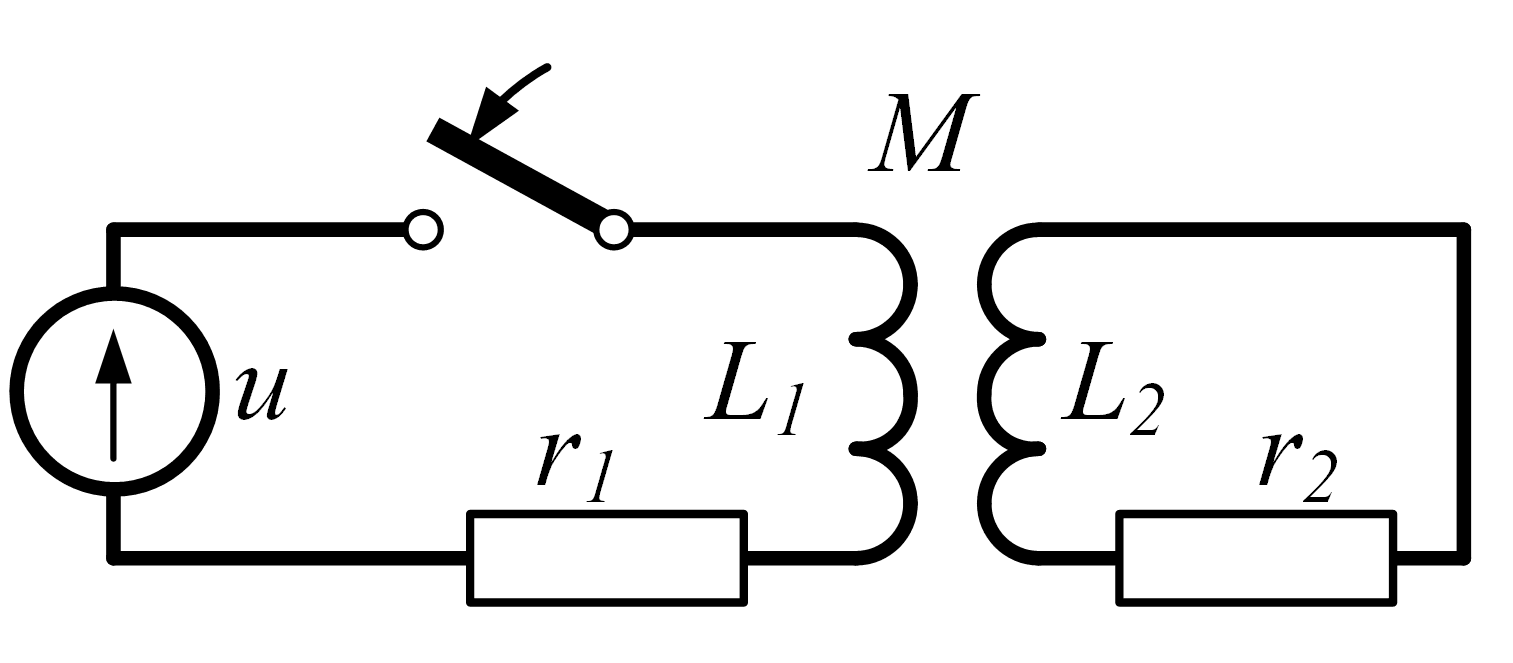
\includegraphics[width=0.40\linewidth]{pic/4-1}
	\caption{Простейшая цепь с магнитной связью.}
	\label{ris:4-1 simplest_circut}
\end{floatingfigure}


\chapter{Установившийся режим короткого замыкания}
\label{chap:5}

\section{Общие замечания}
\label{sec:5-1}


\section{Основные характеристики и параметры}
\label{sec:5-2}


\section{Приведение цепи ротора к статору}
\label{sec:5-3}


\section{Влияние и учет нагрузки}
\label{sec:5-4}


\section{Расчет при отсутствии автоматического регулирования возбуждения}
\label{sec:5-5}


\section{Влияние автоматического регулирования возбуждения}
\label{sec:5-6}

Снижение напряжения, вызванное коротким замыканием. приводит в действие АРВ генераторов, и их возбуждение соответственно возрастает. Поэтому можно заранее предвидеть, что токи и напряжения при этих условиях всегда больше, чем при отсутствии АРВ. Степень такого увеличения зависит от удаленности короткого замыкания и параметров самих генераторов.

В самом деле, если при относительно удаленном коротком замыкании для восстановления напряжения генератора до нормального достаточно лишь немного увеличить возбуждение, то по мере уменьшения удаленности для этого, очевидно, требуется все большее возбуждение. Однако рост последнего у генератора ограничен известным пределом $ I_{f\text{пр}} $.

Следовательно, для каждого генератора можно установить наименьшую величину внешней реактивности, при коротком замыкании за которой генератор при предельном возбуждении обеспечивает нормальное напряжение на своих выводах. Такую реактивность назовем \so{критической реактивностью} $ x_{\text{кр}} $, a связанный с ней очевидным равенством ток

\begin{equation}
    \label{eq:5-16 I_kr}
    I_{\text{кр}}=\frac{U_{\text{н}}}{x_{\text{кр}}}
\end{equation}

--- \so{критическим током}.

Если внешняя реактивность меньше критической, то, несмотря на работу генератора с предельным возбуждением, его напряжение все равно остается ниже нормального. Когда же внешняя реактивность больше критической, то напряжение генератора достигает нормального значения при возбуждении, меньшем предельного.

Таким образом, при коротком замыкании генератор с АРВ в зависимости от внешней реактивности может работать только в одном из двух режимов -- \so{предельного возбуждения} или \so{нормального напряжения}. Лишь в частном случае, когда $ x_{\text{вн}} = x_{\text{кр}} $, оба режима существуют одновременно. Критерием для оценки возможности того или иного режима служит критическая реактивность, величина которой может быть определена по \colorbox{red}{(5-14)}, где следует положить $ E_q = E_{q\text{пр}} $, т.~е.

% остановился 2017-08-30

\section{Расчет при наличии автоматического регулирования возбуждения}
\label{sec:5-7}

В схеме с несколькими генераторами, ток от которых поступает по общим для них ветвям, понятие внешней реактивности по отношению к каждому из них уже теряет смысл. Поэтому здесь нельзя непосредственно использовать установленный в предыдущем параграфе критерий для однозначного определения возможного режима работы каждого генератора при рассматриваемом коротком замыкании. В данном случае расчет приходится вести путем последовательного приближения, задаваясь для генераторов с АРВ в зависимости от положения каждого из них относительно места короткого замыкания либо режимом предельного возбуждения (т.~е. вводя такой генератор в схему своими $ E_{q\text{пр}} $ и $ x_d $), либо режимом нормального напряжения (т.~е. принимая для такого генератора $ E=U_{\text{н}} $ и $ x=0 $) и делая затем проверку выбранных режимов. Последняя заключается в сопоставлении найденных для этих генераторов токов с их критическими токами. Для режима предельного возбуждения должно быть $ I \geqslant I_{\text{кр}} $  (или, иначе, $ U \leqslant U_{\text{н}} $), а для режима нормального напряжения $ I \leqslant I_{\text{кр}} $.

Если в результате проверки оказалось, что режимы некоторых генераторов выбраны неверно, то после их замены нужно сделать повторный расчет с последующей проверкой. При использовании расчетной модели такие пробы выполняются очень быстро. Однако и при аналитическом расчете в большинстве случаев удается с первого раза правильно выбрать режимы генераторов с АРВ. Для этого нужно внимательно проанализировать условия работы отдельных генераторов при рассматриваемом коротком замыкании. В первую очередь нужно установить возможный режим ближайшего к месту короткого замыкания генератора, и если оказывается, что для него должен быть принят режим предельного возбуждения, то следует перейти к оценке возможных режимов других генераторов (или станций), рассматривая их поочередно в порядке увеличения их удаленности. Как только выявлен генератор (или станция), находящийся в режиме нормального напряжения, все приключенные к нему элементы, которые не образуют пути для тока к месту короткого, могут быть отброшены. Это может существенно упростить схему.

Нагрузки увеличивают проводимость приключенной к генератору цепи и, как показано в примере \colorbox{green}{5-4}, могут влиять на режим его работы в условиях короткого замыкания. Это обстоятельство нужно учитывать при оценке возможного режима генераторов с АРВ.

Генераторы без АРВ вводят в схему, как обычно, своими реактивностями $ x_d $ и э.~д.~с. $ E_{q\text{пр}} $ которые у них были в предшествующем режиме. Наличие таких генераторов, вообще говоря, также может повлиять на режим работы генераторов с АРВ.

Все высказанные соображения наглядно иллюстрированы в приводимом ниже конкретном примере.
\chapter{Начальный момент внезапного нарушения режима}
\label{chap:6}

\section{Общие замечания}
\label{sec:6-1}

Прежде чем перейти к знакомству с общими уравнениями электромагнитного переходного процесса синхронной машины, рассмотрим сначала начальный момент такого процесса. Разумеется, все величины в начальный момент внезапного нарушения режима можно получить из упомянутых уравнений как их частное решение для $ t = 0$. Более того, поскольку индуктивности цепей исключают внезапное изменение тока, то значение последнего в начальный момент переходного процесса, вообще говоря, является известным: оно сохраняется таким, что и в конце заданного предшествующего режима. Однако при изменившихся условиях этот ток состоит уже из новых слагающих, которые возникают в данном переходном процессе.

Поскольку поставленная задача ограничена рассмотрением лишь начального момента, вращение ротора и обусловленное этим изменение индуктивностей машины, очевидно, не играют никакой роли. Другими словами, в данном случае машину можно рассматривать как трансформатор.

Исследование начального момента переходного процесса проще и нагляднее вести на основе принципа сохранения первоначального потокосцепления. В самом деле, коль скоро магнитный поток, сцепленный с ротором, в момент внезапного нарушения режима сохраняется неизменным, то соответствующая ему э.~д.~с., наведенная в статоре, в тот же момент также остается неизменной. Следовательно, для синхронной машины условия в начальный момент переходного процесса аналогичны тем же условиям для трансформатора, питаемого источником синусоидального напряжения.

Таким образом, можно предвидеть, что при переходном процессе ток статора синхронной машины состоит из двух слагающих, а именно: \so{периодической}, которая вызывается э.~д.~с., наводимой потоком ротора, и \so{апериодической}, обусловленной изменением потока статора.

Часто рассматривают внезапное изменение тока, имея в виду изменение лишь одной из его слагающих. При этом другие слагающие обеспечивают в момент нарушения режима сохранение предшествующего мгновенного значения тока.

Во всех дальнейших выкладках (как в данной главе, так и в последующих главах) условимся считать:

% TO-DO: этот список должен быть буквенным
\begin{enumerate} 
	\item
	продольную составляющую тока статора положительной, когда создаваемая ею н.~с. совпадает по направлению с н.~с. тока возбуждения;
	\item
	поперечную составляющую тока статора положительной, когда создаваемая ею н.~с. отстает на 90\textdegree (электрических) от н.~с. тока возбуждения; при наличии на роторе поперечного контура это же направление принимается положительным для его магнитной оси;
	\item
	все величины ротора приведенными к статору, причем они, как и все величины статора, выражены в относительных единицах.
\end{enumerate}

Установим теперь, какими э.~д.~с. и реактивностями можно характеризовать синхронную машину в начальный момент переходного процесса.

\section{Переходные э.~д.~с. и реактивности синхронной машины}
\label{sec:6-2}

Обратимся к балансу магнитных потоков в продольной оси ротора синхронной машины при установившемся симметричном режиме ее работы с отстающим по фазе током (\colorbox{red}{рис.~6-1,~а}). При отсутствии насыщения каждый из потоков и их отдельные составляющие можно рассматривать независимо один от другого. Так, полный поток обмотки возбуждения $ \overset{\;.}{\Phi}_f $, который был бы при холостом ходе машины, состоит из полезного потока $ \overset{\;.}{\Phi}_{fad} $ и потока рассеяния $ \overset{\;.}{\Phi}_{\sigma f} $. В свою очередь полезный поток $ \overset{\;.}{\Phi}_{fad} $ является геометрической разностью продольного потока в воздушном зазоре $ \overset{\;.}{\Phi}_{\sigma d} $ и потока продольной реакции статора $ \overset{\;.}{\Phi}_{ad} $. Результирующий магнитный поток $ \overset{\;.}{\Phi}_{f\sum} $, сцепленный с обмоткой возбуждения, складывается из потока $ \overset{\;.}{\Phi}_{\sigma d} $ и потока рассеяния $ \overset{\;.}{\Phi}_{\sigma f} $.

Рассмотрим, как изменится этот баланс, если предположить внезапное изменение, например увеличение потока продольной реакции статора на $ \Delta \overset{\;.}{\Phi}_{ad/0/} $. При этом будем считать, что кроме обмотки возбуждения никаких других контуров в продольной оси ротора не имеется.

В соответствии с законом Ленца приращение потока $ \Delta \overset{\;.}{\Phi}_{ad/0/} $ вызовет ответную реакцию обмотки возбуждения $ \Delta \overset{\;.}{\Phi}_{f/0/} $, причем приращения потокосцеплений $ \Delta \overset{\;.}{\Psi }_{ad/0/} $ и $ \Delta \overset{\;.}{\Psi }_{ad/0/} $ должны компенсировать друг друга, т.~е.

\section{Сверхпереходные э.~д.~с. и реактивности синхронной машины}
\label{sec:6-3}


\section{Сравнение реактивностей синхронной машины}
\label{sec:6-4}


\section{Характеристики двигателей и нагрузки}
\label{sec:6-5}


\section{Практический расчет начального сверхпереходного и ударного токов}
\label{sec:6-6}
\chapter{Уравнения электромагнитного переходного процесса синхронной машины}
\label{chap:7}

\section{Общие замечания и допущения}
\label{sec:7-1}

Ранее уже отмечалось, что аналитическое исследование электромагнитного переходного процесса синхронной машины с учетом всех влияющих на него факторов представляет чрезвычайно сложную задачу. Чтобы несколько упростить ее, приходится вводить ряд допущений, придавая машине некоторые свойства и качества, которыми она в действительности не обладает, т.~е. рассматривать в известной мере «идеализированную» машину. Несомненно, это вносит погрешности в оценку отдельных величин, однако, как показывает сопоставление получаемых величин с экспериментальными данными, обычно погрешности находятся в практически допустимых пределах. Следует особо подчеркнуть, что возможность использования тех или иных конкретных допущений зависит главным образом от характера и назначения решаемой задачи.

В §~\ref{sec:2-1}{2-1} были изложены основные допущения, обычно принимаемые в практических расчетах электромагнитных переходных процессов. Представляется полезным повторить некоторые из них и отметить часть дополнительных допущений, которые используются в дальнейшем. К таким допущениям нужно отнести следующие:

\begin{enumerate} 
	\item
	Магнитная система машины иенасыщена, в силу чего индуктивности машины не зависят от н.~с. (или токов); величины самих индуктивностей при этом определяются для некоторого значения магнитной проницаемости стали магнитопровода.
	\item
	Вместо действительных кривых распределения н.~с. и индукции в воздушном зазоре по расточке статора принимают только их основные, первые гармонические, соответственно чему наведенные в статоре э.~д.~с. выражаются синусоидами основной частоты.
	\item
	В магнитной системе машины отсутствуют какие-либо потери.
	\item
	Конструктивное выполнение машины обеспечивает полную симметрию фазных обмоток статора. Равным образом ротор также симметричен относительно своих продольной и поперечной осей.
	\item
	Предполагается, что как специально созданная продольная демпферная обмотка, так и все прочие естественные демпферные контуры, которые могут быть в продольной оси ротора, заменены одной эквивалентной продольной демпферной обмоткой; аналогично предполагается, что в поперечной оси ротора также имеется только одна эквивалентная поперечная демпферная обмотка\footnote{Для турбогенераторов при более точном анализе требуется учет нескольких демпферных контуров в каждой оси ротора.}.
	\item
	Скорость вращения ротора машины в течение рассматриваемого переходного процесса постоянна и равна синхронной.
\end{enumerate}

Даже для такой идеализированной машины анализ переходного процесса сопряжен со значительными трудностями, для преодоления которых приходится идти еще на некоторые упрощения. Сущность последних будет указана по ходу изложения.

Математические выкладки при учете демпферных обмоток значительно сложнее, и за громоздкостью получающихся выражений труднее понять их физический смысл. Поэтому вначале ограничимся рассмотрением машины без демпферных обмоток. Учет последних сделаем позднее, при этом для упрощения отступим от строгости самих выкладок и используем уже полученные в \href{chap:4}{гл.~4} результаты.

\section{Исходные уравнения}
\label{sec:7-2}


\section{Индуктивности обмоток синхронной машины}
\label{sec:7-3}


\section{Обобщенный вектор трехфазной системы}
\label{sec:7-4}


\section{Замена переменных}
\label{sec:7-5}


\section{Преобразование уравнений}
\label{sec:7-6}


\section{Выражения в операторной форме}
\label{sec:7-7}
\chapter{Форсировка возбуждения и развозбуждение синхронной машины}
\label{chap:8}

\section{Общие замечания}
\label{sec:8-1}

Одной из наиболее эффективных и в то же время простых мер обеспечения надежности работы синхронных машин в большинстве аварийных условий является быстрое повышение их возбуждения или, как говорят, \so{быстродействующая форсировка возбуждения}. В зависимости от принятой системы возбуждения эффективность форсировки различна, что обусловливается особенностями выполнения каждой системы возбуждения. Это различие проявляется в возможных предельных величинах (потолках) токов возбуждения, а также в величинах скоростей нарастания тока возбуждения (принужденного).

Исследование переходного процесса при форсировке возбуждения в общем виде с учетом всех влияющих факторов очень сложно и практически выполнимо лишь с применением современной вычислительной техники. Существенное влияние на форсировку возбуждения оказывает насыщение магнитных систем как самой синхронной машины, так и элементов системы возбуждения. Это обстоятельство делает данную задачу нелинейной со всеми вытекающими отсюда затруднениями.

Несмотря на высказанные замечания, все же представляется целесообразным, даже на базе ранее принятых допущений (см.~§\ref{sec:2-1 osnovnye dopushcheniia}), рассмотреть процесс форсировки возбуждения и понять главным образом физическую сущность происходящих при этом явлений. Свою задачу ограничим случаями, когда машина имеет обычную электромашинную или ионную систему возбуждения. Здесь уместно подчеркнуть, что выбор той или иной системы возбуждения требует всестороннего подхода с различных точек зрения при одновременном учете ряда требований общего и специального характера.

Анализ переходного процесса при развозбуждении или гашении магнитного поля синхронной машины относительно проще, хотя бы уже по той причине, что этот процесс происходит, как правило, после отключения машины от сети. При этом насыщение магнитной системы сказывается также заметно, но даже при пренебрежении им можно получить достаточно правильное представление о протекании такого процесса.

В дальнейшем, так же как и в \ref{chap:7}{гл.~7}, предполагается, что все величины цепей ротора приведены к статору и выражены в системе относительных единиц. Для упрощения записи специальные обозначения, указывающие такое приведение, опущены.

\section{Включение обмотки возбуждения на постоянное напряжение}
\label{sec:8-2}


\section{Форсировка возбуждения при электромашинном возбудителе}
\label{sec:8-3}


\section{Форсировка при управляемых ионных и тиристорных системах возбуждения}
\label{sec:8-4}

В последнее время широкое применение находят ионные и тиристорные системы возбуждения\footnote{Ведутся работы по созданию бесщеточных систем возбуждения; их динамические характеристики находятся в стадии исследования.}; при этом используют управляемые ионные или тиристорные выпрямители.

Ионные и тиристорные системы возбуждения позволяют легко обеспечить при форсировке очень быстрое нарастание напряжения возбуждения и большую предельную величину последнего. Это достигается обычно установкой двух выпрямителей, включенных параллельно. Один из них обеспечивает возбуждение машины в нормальном режиме, а другой служит для форсировки возбуждения. Регулирование возбуждения машины в нормальных условиях производят, используя систему управления выпрямителей.

Поскольку ионные и тиристорные системы возбуждения практически безынерционны ($ T_e \approx 0,02\text{~сек.} $), можно считать, что при форсировке возбуждения напряжение на кольцах обмотки возбуждения синхронной машины возрастает до предельного $ u_{f\text{пр}} $ скачком. Поэтому все выражения, полученные ранее для форсировки возбуждения при электромашинном возбудителе, применимы и при указанных системах возбуждения, для чего достаточно положить в них $ T_e = 0 $; это приводит к значительному их упрощению.

\section{Гашение магнитного поля}
\label{sec:8-5}
\chapter{Внезапное короткое замыкание синхронной машины}
\label{chap:9}

\section{Общие замечания}
\label{sec:9-1}

Анализ электромагнитного переходного процесса при внезапном коротком замыкании, рассматриваемый в настоящей главе, ограничен условием, что синхронная машина работает отдельно от других источников питания. Внешняя цепь ее статора при возникшем коротком замыкании характеризуется некоторым постоянным сопротивлением, преимущественно индуктивным.

Чтобы иметь некоторое представление о взаимном влиянии машин на характер протекания электромагнитного переходного процесса (при неизменной скорости их вращения), в конце главы данный вопрос кратко освещен для простейших условий, когда в схеме имеются две машины, связанные между собой через произвольные реактивности.

Вначале рассматривается переходный процесс в синхронной машине без демпферных обмоток и при отключенном устройстве автоматического регулирования возбуждения. В дальнейшем введен учет такого регулирования, используя материал предыдущей главы. Влияние и

учет демпферных обмоток изложен без строгих математических выкладок; при этом основное внимание обращено на вскрытие физической сущности явления и возможности упрощенной оценки этого влияния.

Практический интерес представляет протекание процесса при каскадном (или ступенчатом) отключении короткого замыкания и его повторном включении. В общем виде данный вопрос очень сложен. Поэтому здесь он рассмотрен применительно к условиям, когда в схеме имеется лишь одна машина.

\section{Внезапное короткое замыкание синхронной машины без демпферных обмоток}
\label{sec:9-2}


\section{Влияние и приближенный учет демпферных обмоток}
\label{sec:9-3}

Общий путь исследования электромагнитного переходного процесса внезапного короткого замыкания синхронной машины с демпферными обмотками принципиально тот же, что и в предыдущем параграфе. Такая машина характеризуется операторными реактивностями в обеих осях ротора. Каждая дополнительная обмотка на роторе повышает порядок определителя системы уравнений, аналогичной (9-7) и (9-8). Так, если по осям $ d $ и $ q $ расположено по одной демпферной обмотке, то $ p $ в определителе уже достигает пятой степени. При этом решение характеристического уравнения, получающегося путем приравнивания определителя нулю, в общем виде невозможно. Достаточно близкое к действительности решение можно получить, так же как и при отсутствии демпферных обмоток, пренебрегая поочередно активными сопротивлениями цепей ротора и статора.

При таком решении корни характеристического уравнения $ p_1 $ и $ p_2 $ могут быть определены по (9-12), где вместо $ x'_d $ и $ x_q $ нужно ввести соответственно $ x''_d $ и $ x''_q $. Для нахождения значений $ T_a $ и $ x_2 $ должна быть сделана аналогичная замена в (9-13) и (9-14).


\section{Влияние автоматического регулирования возбуждения при внезапном коротком замыкании}
\label{sec:9-4}


\section{Каскадное отключение и повторное включение короткого замыкания}
\label{sec:9-5}


\section{Взаимное электромагнитное влияние синхронных машин при переходном процессе}
\label{sec:9-6}
\chapter{Практические методы расчета переходного процесса короткого замыкания}
\label{chap:10}

\section{Общие замечания}
\label{sec:10-1}

Полученные в гл.~\ref{chap:9} общие выражения для тока при внезапном коротком замыкании позволяют с высокой точностью определить его величину в произвольный момент переходного процесса в цепи, питаемой одним генератором. Структура этих выражений показывает, что даже при столь простых условиях их применение требует большой вычислительной работы.

При переходе к схемам с несколькими генераторами, как показано в §~\ref{sec:9-6}, задача точного расчета переходного процесса короткого замыкания резко усложняется. Оставляя в стороне вопросы учета возникающих качаний генераторов и поведения присоединенных нагрузок, достаточно вспомнить, что изменения свободных токов в каждом из генераторов взаимно связаны между собой. При автоматическом регулировании возбуждения аналогичная связь имеет место также в приращениях принужденных токов. Трудность точного расчета дополнительно усугубляется различием параметров синхронной машины в продольной и поперечной осях ее ротора.

Использование приемов операционного исчисления для расчета переходных процессов короткого замыкания в мало-мальски сложной схеме сопряжено с преодолением весьма громоздких и трудоемких выкладок. Порядок характеристического уравнения быстро возрастает с увеличением числа машин в рассматриваемой схеме. Поэтому практическое применение такого метода расчета весьма ограничено. Его можно рассматривать лишь как эталон для оценки других приближенных методов расчета.

В силу указанных причин и с учетом того, что для решения многих практических задач не требуется знания точных результатов, разработаны приближенные методы расчета переходного процесса короткого замыкания. В дальнейшем рассмотрены только те из них, которые достаточно широко используются главным образом в практике советской электроэнергетики.

Основное требование, которому должен удовлетворять практический метод, заключается в простоте его выполнения, что прежде всего предотвращает возможность ошибок. Однако чем проще метод, тем на большем числе допущений он основан и тем, очевидно, меньше его точность. Самые простые методы позволяют иногда определить лишь порядок искомых величин, но этого часто бывает достаточно, чтобы обоснованно решить некоторые практические задачи. Почти, как правило, можно рекомендовать начать расчет переходного процесса короткого замыкания самым простым методом, а затем, если это требуется, вводить уточнения.

Помимо ранее указанных допущений (см.§~\ref{sec:2-1}), в практических расчетах коротких замыканий дополнительно принимают, что:

% остановился 2017-08-29

\section{Приближенный учет системы}
\label{sec:10-2}


\section{Расчет для выбора выключателей по отключающей способности}
\label{sec:10-3}


\section{Метод расчетных кривых}
\label{sec:10-4}


\section{Уточнение метода расчетных кривых}
\label{sec:10-5}


\section{Метод спрямленных характеристик}
\label{sec:10-6}
\part{Электромагнитные переходные процессы при нарушении симметрии трехфазной цепи}

\chapter{Основные положения в исследовании несимметричных переходных процессов}
\label{chap:11}

\section{Общие замечания}
\label{sec:11-1}


\section{Образование высших гармоник}
\label{sec:11-2}


\section{Применимость метода симметричных составляющих к исследованию переходных процессов}
\label{sec:11-3}
\chapter{Параметры элементов для токов обратной и нулевой последовательностей}
\label{chap:12}

\section{Общие замечания}
\label{sec:12-1}

Все сопротивления, которыми характеризуются отдельные элементы в нормальном симметричном режиме, а также в симметричном переходном процессе, по существу являются сопротивлениями прямой последовательности\footnote{Исключение составляет реактивность, используемая при определении постоянной времени $ T_a $ (см~§ \ref{chap:9-2})}. Этот термин вводить ранее не было нужды, поскольку токи были лишь одной последовательности.

При отсутствии магнитной связи между фазами какого-либо элемента его сопротивление не зависит от порядка чередования фаз тока. Активная и реактивная слагающие сопротивления такого элемента зависят только от частоты тока и, следовательно, для всех последовательностей одинаковы\footnote{Такими элементами можно практически считать реакторы}, т. е.

\begin{equation*}
	r_1 = r_2 = r_0
\end{equation*}

и

\begin{equation*}
	x_1 = x_2 = x_0
\end{equation*}

соответственно

\begin{equation*}
	z_1 = z_2 = z_0
\end{equation*}

Для элемента, магнитносвязанные цепи которого неподвижны относительно друг друга, сопротивления прямой и обратной последовательностей одинаковы, так как от перемены порядка чередования фаз симметричной трехфазной системы токов взаимоиндукция между фазами такого элемента не изменяется.

Таким образом, для трансформаторов, автотрансформаторов, воздушных линий, кабелей и реакторов

\begin{equation*}
	r_1 = r_2
\end{equation*}

и

\begin{equation*}
	x_1 = x_2
\end{equation*}

соответственно

\begin{equation*}
	z_1 = z_2
\end{equation*}

Система токов нулевой последовательности резко отличается от систем токов прямой и обратной последовательностей, вследствие чего сопротивления нулевой последовательности в общем случае весьма существенно отличаются от соответствующих сопротивлений двух других последовательностей.

Помимо определения индуктивных сопротивлений обратной и нулевой последовательностей, ниже также приведены указания к определению активных сопротивлений нулевой последовательности воздушных и кабельных линий. Учет последних часто необходим при расчете однофазных коротких замыканий, причем его выполнение обычно не вызывает трудностей, так как этот вид короткого замыкания в большинстве случаев характеризуется большой электрической удаленностью, что позволяет не считаться с изменением тока во времени.

\section{Синхронные машины}
\label{sec:12-2}

Магнитный поток, созданный токами обратной последовательности синхронной частоты, вращаясь относительно ротора с двойной синхронной скоростью, встречает на своем пути непрерывно изменяющееся магнитное сопротивление; это обусловлено магнитной несимметрией ротора и тем, что наведенные в продольных и поперечных контурах ротора токи создают различные ответные реакции. Таким образом, при неизменной н.~с. статора поток обратной последовательности гармонически изменяется с двойной синхронной скоростью в пределах между его наибольшим и наименьшим значениями, разница между которыми зависит от степени несимметрии ротора; она велика при резкой несимметрии ротора и, напротив, совсем исчезает при его полной симметрии.

В §\ref{sec:11-2} было показано, что поток обратной последовательности синхронной частоты в общем случае вызывает в статоре нечетные гармоники, которые искажают синусоидальную форму магнитного поля статора. Это обстоятельство существенно затрудняет определение реактивности обратной последовательности синхронной машины и приводит к тому, что данная реактивность, строго говоря, не является параметром машины, так как она зависит от внешних условий (т.~е. внешней реактивности, вида несимметрии и др.).

Для синхронной машины без демпферных обмоток в §~\ref{sec:9-2} было получено выражение для реактивности

\begin{equation}
	x_2 = \frac{2x'_d x_q}{x'_d + x_q} \text{,}
	\label{eq:12-1}
\end{equation}

которая по существу представляет собой реактивность обратной последовательности, определяемую как отношение подведенного синусоидального напряжения обратной последовательности синхронной частоты к основной гармонике тока обратной последовательности.

Эта реактивность может быть представлена схемой замещения, показанной на рис.~\ref{fig:12-1}. Ток в параллельной ветви с реактивностью дает значение третьей гармоники тока прямой последовательности, которая вызвана потоком обратной последовательности синхронной частоты.

Представим себе теперь, что напряжение обратной последовательности приложено не непосредственно к статору машины, а через произвольную реактивность $ x $. Тогда общая реактивность обратной последовательности всей цепи, очевидно, будет:

\begin{equation*}
	x_{2\Sigma}  = \frac{2(x'_d + x) (x_q + x)}{x'_d + x_q + 2x}
\end{equation*}

и на долю самой машины приходится величина

\begin{equation*}
	x_{2}  = \frac{2(x'_d + x) (x_q + x)}{x'_d + x_q + 2x} - x = \frac{2x'_d x_q + (x'_d + x_q) x}{x'_d + x_q + 2x} \text{,}
\end{equation*}

которая, как видно, зависит от внешней реактивности $ x $. По мере увеличения последней реактивность обратной последовательности машины стремится в пределе к

\begin{equation}
	x_{2}  = \lim_{x \rightarrow \infty } = \frac{2x'_d x_q + (x'_d + x_q) x}{x'_d + x_q + 2x} = \frac{x'_d + x_q}{2} \text{,}
	\label{eq:12-2}
\end{equation}

что соответствует отсутствию третьей гармоники тока. Эта реактивность получается из схемы замещения рис.~\ref{fig:12-1}, для чего достаточно разомкнуть рубильник \textit{Р}.

\begin{wrapfigure}{l}{0.5\linewidth} %\begin{wrapfigure}[высота в строках]]{r}{0.4\linewidth} % 1-1
	\centering
	\includesvg{pic/12-1}
	\caption{Схема замещения, определяющая реактивность $ x_2 $ синхронной машины с учетом влияния третьей гармоники тока прямой последовательности}
	\label{fig:12-1}
\end{wrapfigure}

Следовательно, принципиальная разница между выражениями (\ref{eq:12-1}) и (\ref{eq:12-2}) состоит в том, что первое из них дает значение $ х_2 $ машины с учетом влияния третьей гармоники тока, а второе -- без учета такого влияния. При симметричном роторе ($ х_q = х'_d $) оба выражения дают одно и тоже значение что также следует из схемы замещения рис.~\ref{fig:12-1}.

До сих пор предполагалось, что обратно-синхронное питание подано от источника бесконечной мощности, в силу чего, помимо основной гармоники, в статоре возникает еще только третья гармоника тока. Однако при несимметричном режиме машины (см.~§~\ref{sec:11-2}) поле обратной последовательности основной частоты вызывает в статоре весь спектр нечетных гармоник. В этом случае, как показал Н.~Н.~Щедрин, схема замещения рис.~\ref{fig:12-1} может быть развита в бесконечную цепную схему замещения, результирующая реактивность которой составляет:

\begin{equation}
	x_{2}  = \sqrt{x'_d x_q} \text{.}
	\label{eq:12-3}
\end{equation}

Эта реактивность также зависит от внешней реактивности и в пределе стремится к значению, определяемому по (\ref{eq:12-2}).

Для машины с демпферными обмотками реактивность $ x_2 $ может быть определена по тем же выражениям, если заменить в них $ x'_d $ и $ x_q $ соответственно $ x''_d $ и $ x''_q $. Величины реактивностей $ x''_d $ и $ x''_q $ обычно ближе друг к другу, чем величины $ x'_d $ и $ x_q $. Поэтому у машин с полным демпфированием разница в значениях $ x_2 $, получаемых по разным выражениям, очень мала.

Поскольку выражения (\ref{eq:12-1}) -- (\ref{eq:12-3}) почти равноценны, в большинстве практических расчетов целесообразно принимать для синхронных машин реактивность $ x_2 $ по наиболее простому выражению (\ref{eq:12-2}), которое к тому же удовлетворяет нормальному правилу последовательного соединения реактивностей машины и ее внешней цепи. При необходимости учета высших гармоник надлежит применять более точное выражение (\ref{eq:12-3}).

В качестве приближенных соотношений принимают:

%TODO: как выделить этот долбанный блок?
\begin{tabular}{lc}
	Для машин без демпферных обмоток & $ x_2 \approx 1,45 x'_d  $; \\ 
	Для турбогенераторов и машин с демпферными обмотками в обеих осях ротора &  $ x_2 \approx 1,22 x''_d  $. \\ 
\end{tabular} 

В практических приближенных расчетах обычно идут на дополнительное упрощение, принимая для турбогенераторов и машин с продольно-поперечными демпферными обмотками

\begin{equation}
	x_2 \approx x''_d \text{.}
	\label{eq:12-4}
\end{equation}

Токи нулевой последовательности создают практически только магнитные потоки рассеяния статорной обмотки, которые, как правило, меньше, чем при токах прямой или обратной последовательности, причем это уменьшение сильно зависит от типа обмотки. Поэтому величина $ x_0 $ синхронных машин колеблется в широких пределах:

\begin{equation}
	x_0 = (0,15 \div 0,6) x''_d \text{.}
	\label{eq:12-5}
\end{equation}

\section{Асинхронные двигатели}
\label{sec:12-3}

Если в нормальных условиях асинхронный двигатель работает со скольжением $ s $, то по отношению к магнитному потоку обратной последовательности синхронной частоты ротор двигателя, очевидно, имеет скольжение $ (2-s) $. Следовательно, сопротивление обратной последовательности асинхронного двигателя представляет собой его сопротивление при скольжении $ (2-s) $.

Кривая, показанная на рис.~\ref{fig:12-2}, иллюстрирует примерный характер относительного изменения реактивности асинхронного двигателя в функции скольжения\footnote{За единицу реактивности здесь принята реактивность двигателя при его номинальном скольжении.}.

Как видно, с ростом $ s $ реактивность двигателя вначале резко падает, а затем ее снижение весьма незначительно. Это позволяет практически считать

\begin{equation}
	x_2 \approx x_{s=1} = x_{\text{K}} \text{,}
	\label{eq:12-6}
\end{equation}

т.~е. реактивность $ x_2 $ двигателя равной его так называемой реактивности короткого замыкания (относительная величина которого близка к обратной величине относительного номинального пускового тока).

\begin{figure} %\begin{wrapfigure}[высота в строках]]{r}{0.4\linewidth} % 1-1
	\centering
	\includesvg{pic/12-2}
	\caption{Относительное изменение индуктивного сопротивления асинхронного двигателя в зависимости от скольжения.}
	\label{fig:12-2}
\end{figure}

Реактивность нулевой последовательности асинхронного двигателя, как и синхронных машин, определяется только рассеянием статорной обмотки и сильно зависит от типа и конструкции последней. Достаточно надежные значения этой реактивности могут быть получены преимущественно опытным путем или по данным завода-изготовителя.

\section{Обобщенная нагрузка}
\label{sec:12-4}

Реактивность обратной последовательности обобщенной нагрузки зависит от характера приемников электроэнергии и относительного участия каждого из них в рассматриваемой нагрузке. Для средней типовой промышленной нагрузки можно считать, что основная ее часть состоит из асинхронных двигателей, реактивность обратной последовательности которых, как показано в §~\ref{sec:12-3}, практически та же, что и в начальный момент внезапного нарушения режима. Поэтому для реактивности обратной последовательности обобщенной нагрузки в практических расчетах можно принимать, как и в §~\ref{sec:6-5}, величину

\begin{equation}
	x_2 = 0,35 \text{,}
	\label{eq:12-7}
\end{equation}

считая ее отнесенной к полной рабочей мощности в мегавольтамперах данной нагрузки и среднему номинальному напряжению той ступени, где она присоединена.

Поскольку обобщенная нагрузка включает в себя сеть и понижающие трансформаторы, ее сопротивление нулевой последовательности обычно определяется именно этими элементами, рассмотрение которых приведено ниже. Привести какие-либо средние величины этого сопротивления не представляется возможным.

% https://tex.stackexchange.com/questions/153329/footnote-in-sub-section-title
\section{Трансформаторы\protect\footnote{Для общности проводимых здесь записей обмотки трансформатора обозначены порядковыми номерами І, II, III вместо В, С, Н, как это обычно принято.}}
\label{sec:12-5}

Реактивность нулевой последовательности трансформатора в значительной мере определяется его конструкцией и соединением обмоток.

Со стороны обмотки, соединенной в треугольник или в звезду без заземленной нейтрали, независимо от того, как соединены другие обмотки, реактивность нулевой последовательности трансформатора, очевидно, бесконечно велика ($ x_0 = \infty $), так как при этих условиях вообще исключена возможность циркуляции тока нулевой последовательности в данном трансформаторе. Следовательно, конечная, хотя иногда (см.~ниже) и очень большая, реактивность нулевой последовательности трансформатора может быть только со стороны его обмотки, соединенной в звезду с заземленной нейтралью.

На рис.~\ref{fig:12:3}, \textit{а}, \textit{б} и \textit{в} приведены основные варианты соединения обмоток двухобмоточного трансформатора, при которых приложенное к обмотке \textit{I} напряжение нулевой последовательности вызывает в одной или в обеих обмотках ток той же последовательности. Справа, против каждого варианта соединения обмоток показаны схемы замещения трансформатора (без учета активных сопротивлений) для токов нулевой последовательности.

При соединении обмоток $ \text{Y}_0 / \Delta $ (рис.~\ref{fig:12-3},~\textit{а}) э.~д.~с. нулевой последовательности трансформатора целиком расходуется на проведение тока той же последовательности только через реактивность рассеяния обмотки, соединенной треугольником, так как этот ток (подобно третьей гормонике тока) не выходит за пределы данной обмотки. В схеме замещения это отражают закорачиванием ветви с $ x_{II} $. Потенциал, равный нулю, на конце ветви $ x_{II} $ схемы замещения не указывает на искусственный перенос заземления нейтрали, как это иногда ошибочно воспринимают; он только соответствует условию, что данной ветвью схемы замещения трансформатора заканчивается путь циркуляции токов нулевой последовательности.

При соединении обмоток $ \text{Y}_0 / \text{Y}_0 $ представленная на рис.~\ref{fig:12-3},~\textit{б} схема замещения предполагает, что на стороне обмотки \textit{II} обеспечен путь для тока нулевой последовательности, т.~е. в цепи этой обмотки имеется по меньшей мере еще одна заземленная нейтраль (см.~пунктир). Если же этого нет, то схема замещения будет такой же, как и при соединении обмоток $ \text{Y}_0 / \text{Y} $ (рис.~\ref{fig:12-3},~\textit{в}), что соответствует режиму холостого хода трансформатора.

Оценим теперь величину реактивности намагничивания нулевой последовательности трансформатора $ x_{\mu_0} $.

Для группы из трех однофазных трансформаторов, а также для трехфазных четырех- и пятистержневых (броневых) трансформаторов ток намагничивания нулевой последовательности очень мал, так как в этом случае условия для магнитного потока практически те же, что и при питании трансформатора от источника напряжения прямой (или обратной) последовательности. Поэтому в соответствии с принятым ранее (§~\ref{sec:2-1}) допущением можно считать $ x_{\mu_0} = \infty $.

Иные условия имеют место в трехфазных трехстержневых трансформаторах, где магнитные потоки нулевой последовательности вынуждены замыкаться через изолирующую среду и кожух трансформатора. Для проведения магнитного потока по пути со столь высоким магнитным сопротивлением необходим достаточно большой ток намагничивания; следовательно, реактивность $ x_{\mu_0} $ у трансформатора такого типа значительно меньше, чем $ x_{\mu_1} $. В зависимости от конструкции этого типа трансформатора она находится в пределах $ x_{\mu_0} = (0,3 \div 1,0 ) $. Имея в виду, что величина $ x_{II} $ все же значительно меньше $ x_{\mu_0} $, можно практически считать, что и для трехстержневого трансформатора с соединением обмоток $ \text{Y}_0 / \Delta $ ~~ $ x_{\mu_0} \approx \infty $.

В табл.~\ref{tabl:12-1} сведены изложенные выше указания относительно оценки реактивности нулевой последовательности двухобмоточных трансформаторов.

%TODO: Таблица 12-1

У трехобмоточных трансформаторов одна из обмоток, как правило, соединена в треугольник. Поэтому для них всегда можно принимать $ x_{\mu_0} = \infty $.

Основные варианты соединения обмоток трехобмоточного трансформатора и соответствующие им схемы замещения нулевой последовательности (считая $ U_0 $ приложенным со стороны обмотки \textit{I}) приведены на рис.~\ref{fig:12-3},~\textit{г}, \textit{д} и \textit{e}.

В варианте рис.~\ref{fig:12-3},~\textit{г} ток нулевой последовательности в обмотке \textit{III} отсутствует. Следовательно, в этом случае $ x_0 = x_I + x_{II} + x_{I-II} $.

В варианте рис.~\ref{fig:12-3},~\textit{д} предполагается, что путь для тока нулевой последовательности на стороне обмотки \textit{III} обеспечен. В этом случае в схему нулевой последовательности трансформатор должен быть введен своей схемой замещения.

Наконец, в варианте ~\ref{fig:12-3},~\textit{e} компенсация тока нулевой последовательности обмотки \textit{I} осуществляется токами, наведенными в обмотках \textit{II} и \textit{III}. В этом случае

\begin{equation*}
	x_0 = x_1 + \frac{ x_{II} x_{III} }{ x_{II} + x_{III} } \text{.}
\end{equation*}

\section{Автотрансформаторы\protect\footnote{См.~сноску к §~\ref{sec:12-5}}}
\label{sec:12-6}

Обмотки автотрансформатора связаны между собой не только магнитно, но и электрически; поэтому здесь иные условия для протекания токов нулевой последовательности, которые должны быть отражены в схеме замещения нулевой последовательности автотрансформатора. При известных условиях, как показано ниже, даже при изолированной нейтрали автотрансформатора в его обмотках возможна циркуляция токов нулевой последовательности.

При глухом заземлении нейтрали автотрансформатора его схема замещения нулевой последовательности аналогична схеме соответствующего трансформатора. Так, если у автотрансформатора нет третьей обмотки и во вторичной цепи обеспечен путь для тока нулевой последовательности, его схема замещения (при пренебрежении намагничивающим током и активными сопротивлениями) представляется суммарной реактивностью рассеяния (рис.~\ref{fig:12-4},~\textit{а}). При наличии третьей обмотки\footnote{Силовые автотрансформаторы, как правило, снабжены такой обмоткой}, соединенной треугольником, схема замещения имеет тот же вид, что и у трехобмоточного трансформатора при соответственном соединении его обмоток (рис.~\ref{fig:12-4},~\textit{в}).

Следует подчеркнуть, что непосредственно из схемы замещения нулевой последовательности автотрансформатора нельзя получить ток, протекающий в его нейтрали. При указанных на рис.~\ref{fig:12-4} направлениях токов искомый ток в нейтрали равен утроенной разности токов нулевой последовательности первичной и вторичной цепей, т.~е. $ \overset{~\cdot}{I}_N = 3( \overset{~\cdot}{I}_{0I} - \overset{~\cdot}{I}_{0II}) $, причем каждый из них должен быть отнесен к своей ступени напряжения, а не к какой-либо одной, для которой составлена схема замещения.

%TODO: Рисунок 12-4

Допустим теперь, что нейтраль автотрансформатора заземлена через реактивность $ X_N $ (рис.~\ref{fig:12-4},~\textit{б}). Если напряжение на нейтрали равно $ U_N $ и напряжения выводов ступеней \textit{I} и \textit{II} относительно нейтрали составляют соответственно $ U_{N\text{I}} $ и $ U_{N\text{II}} $ то для результирующей реактивности нулевой последовательности между выводами ступеней \textit{I} и \textit{II} автотрансформатора, приведенной к ступени \textit{I}, можно написать:

\begin{equation*}
	x'_{I-II} = \frac{( U_{N\text{I}} + U_N ) - ( U_{N\text{II}} + U_N ) U_{\text{I}} / U_{\text{II}} }{I_{0\text{I}}} = \frac{ U_{N\text{I}} - \overset{\circ }{U}_{N\text{II}} }{ I_{0\text{I}} } + \frac{U_N}{I_{0\text{I}}}\left ( 1- \frac{U_{\text{I}}}{U_{\text{II}}} \right ) \text{;}
\end{equation*}

поскольку

\begin{equation*}
	\frac{ U_{N\text{I}} - \overset{\circ }{U}_{N\text{II}} }{ I_{0\text{I}} } = x_{\text{I-II}} \text{,}
\end{equation*}

где $ x_{\text{I-II}} $ -- реактивность рассеяния автотрансформатора, отнесенная к ступени \textit{I},

и

\begin{equation*}
	\frac{ U_{N} }{ I_{0\text{I}} } = \frac{ 3x_N ( I_{0\text{I}} - I_{0\text{II}} ) }{ I_{0\text{I}} } = 3x_N \left ( 1- \frac{U_{\text{I}}}{U_{\text{II}}} \right ) \text{,}
\end{equation*}

то окончательно получим:

\begin{equation}
	x'_{\text{I-II}} = x_{\text{I-II}} + 3x_N \left ( 1- \frac{U_{\text{I}}}{U_{\text{II}}} \right )^2 \text{.}
	\label{eq:12-8}
\end{equation}

Данное выражение, разумеется, справедливо также и в том случае, когда реактивности представлены в относительных единицах, причем его запись предполагает, что реактивность $ x_N $ отнесена к базисному напряжению ступени \textit{I}.

Аналогичным образом для автотрансформатора, имеющего третью обмотку, соединенную треугольником (рис.~\ref{fig:12-4},~\textit{г}), нетрудно найти результирующие реактивности нулевой последовательности между другими парами его обмоток, также отнесенные к ступени \textit{I}:

\begin{equation}
	x'_{\text{I-III}} = x_{\text{I-III}} + 3x_N \text{;}
	\label{eq:12-9}
\end{equation}

\begin{equation}
	x'_{\text{I-III}} = x_{\text{II-III}} + 3x_N \left (\frac{U_{\text{I}}}{U_{\text{II}}} \right )^2 \text{.}
	\label{eq:12-10}
\end{equation}

Используя (\ref{eq:12-8}) -- (\ref{eq:12-10}), по известным формулам для трехобмоточного трансформатора (см.~приложение \colorbox{red}{П-7}) находим реактивности трехлучевой схемы замещения:

% промежутки между строк матрицы - https://tex.stackexchange.com/questions/14071
\begin{equation}
	\left.\begin{matrix}
	x'_{\text{I}} = x_{\text{I}} + 3x_N \left ( 1- \frac{U_{\text{I}}}{U_{\text{II}}} \right ) \text{;} \\[1em]
	x'_{\text{II}} = x_{\text{II}} + 3x_N \frac{(U_{\text{I}} - U_{\text{II}})U_{\text{I}}}{U_{\text{II}}^2} \text{;} \\[1em]
	x'_{\text{III}} = x_{\text{III}} + 3x_N \frac{U_{\text{I}}}{U_{\text{II}}} \text{.}
	\end{matrix}\right\}
	\label{eq:12-11}
\end{equation}

У автотрансформатора без третьей обмотки разземление нейтрали приводит к тому, что в схеме нулевой последовательности такой автотрансформатор оказывается в режиме холостого хода; его ток намагничивания достаточно мал и им можно пренебречь, поэтому $ x_{\mu_0} = \infty $.

Иные условия имеют место при разземлении нейтрали автотрансформатора, который снабжен третьей обмоткой, соединенной треугольником. В этом случае циркуляция тока нулевой последовательности возможна \cite{04Ulianov64}.





















\section{Воздушные линии}
\label{sec:12-7}


\section{Кабели}
\label{sec:12-8}
\chapter{Схемы отдельных последовательностей}
\label{chap:13 skhemy_otdelnykh_posledovatelnostei}

\section{Общие замечания}
\label{sec:13-1 obshchie_zamechaniia}

При применении метода симметричных составляющих к расчету любого несимметричного режима или процесса одной из первоочередных задач является составление схем замещения в общем случае всех трех последовательностей (прямой, обратной и нулевой).

При аналитическом решении поставленной задачи по этим схемам находят результирующие сопротивления отдельных последовательностей рассматриваемой системы относительно места, где возникла несимметрия. Из схемы замещения прямой последовательности, помимо того, находят результирующую э.~д.~с. относительно той же точки.

Когда используют расчетные модели (или столы), надобность в определении таких результирующих величин отпадает, так как в этом случае после объединения схем замещения отдельных последовательностей в комплексную схему для рассматриваемого вида несимметрии (см. \colorbox{red}{§ 14-7 и 15-6}) токи и напряжения отдельных последовательностей можно найти в некотором масштабе по показаниям измерительных приборов.

Схемы замещения отдельных последовательностей составляют, как обычно, в соответствии с указаниями \colorbox{red}{§ 2-4}. В частности, элементы схем замещения выражают в именованных или относительных единицах, приводя соответственно к выбранной основной ступени напряжения или к выбранным базисным условиям.

\section{Схемы прямой и обратной последовательности}
\label{sec:13-2 skhemy_priamoi_i_obratnoi_posledovatelnosti}

Схема прямой последовательности является обычной схемой, которую составляют для расчета любого симметричного трехфазного режима или процесса. В зависимости от применяемого метода расчета и момента времени в нее вводят генераторы и нагрузки соответствующими реактивностями и э.~д.~с. Все остальные элементы вводят в схему неизменными сопротивлениями.

Поскольку пути циркуляции токов обратной последовательности те же, что и токов прямой последовательности, схема обратной последовательности по структуре аналогична схеме прямой последовательности. Различие между ними состоит прежде всего в том, что в схеме обратной последовательности э.~д.~с. всех генерирующих ветвей условно принимают равными нулю (см. \colorbox{red}{§ 11-3}); кроме того, считают, что реактивности обратной последовательности синхронных машин и нагрузок практически постоянны и не зависят от вида и условий возникшей несимметрии, а также от продолжительности переходного процесса.

\so{Началом схемы прямой или обратной последовательности} считают точку, в которой объединены свободные концы всех генерирующих и нагрузочных ветвей; это точка нулевого потенциала схемы соответствующей последовательности.

\so{Концом схемы прямой или обратной последовательности} считают точку, где возникла рассматриваемая несимметрия. При продольной несимметрии каждая из схем имеет два конца; ими являются две точки, между которыми расположена данная продольная несимметрия. К концу или между концами схем отдельных последовательностей приложены напряжения соответствующих последовательностей, возникающие в месте несимметрии.

\section{Схема нулевой последовательности}
\label{sec:13-3 skhema_nulevoi_posledovatelnosti}

Токи нулевой последовательности по существу являются однофазным током, разветвленным между тремя фазами и возвращающимся через землю и параллельные ей цепи. В силу этого путь циркуляции токов нулевой последовательности резко отличен от пути, по которому проходят токи прямой или обратной последовательности.

Схема нулевой последовательности в значительной мере определяется соединением обмоток участвующих трансформаторов и автотрансформаторов.

\textit{Составление схемы нулевой последовательности следует начинать, как правило, от точки, где возникла несимметрия, считая, что в этой точке все фазы замкнуты между собой накоротко и к ней приложено напряжение нулевой последовательности.} В зависимости от вида несимметрии это напряжение прикладывается или относительно земли (поперечная несимметрия, \colorbox{red}{рис. 13-1,\textit{а}}) или последовательно, в рассечку фазных проводов (продольная несимметрия, \colorbox{red}{рис. 13-1,\textit{6}}).

Исходя из соответствующего данной несимметрии включения напряжения нулевой последовательности, далее следует выявить в пределах каждой электрически связанной цепи возможные пути протекания токов нулевой последовательности.

Когда напряжение нулевой последовательности приложено относительно земли, то при отсутствии емкостной проводимости для циркуляции токов нулевой последовательности необходима по меньшей мере одна заземленная нейтраль в той же электрически связанной цепи, где приложено это напряжение. При нескольких заземленных нейтралях в этой цепи образуется соответственно несколько параллельных контуров для токов нулевой последовательности.

При продольной несимметрии, т. е. когда напряжение нулевой последовательности введено последовательно, в фазные провода, циркуляция токов нулевой последовательности возможна даже при отсутствии заземленных нейтралей, если при этом имеется замкнутый контур через обходные пути той же электрически связанной цепи \footnote{При этом в земле циркулирует наведенный ток, следуя по трассе линии.}. При отсутствии таких путей протекание токов нулевой последовательности в рассматриваемых условиях возможно только в том случае, если в той же электрически связанной цепи имеются заземленные нейтрали с обеих сторон от места, где приложено напряжение нулевой последовательности.

\textit{Сопротивление, через которое заземлена нейтраль трансформатора, генератора, двигателя, нагрузки, должно быть введено в схему нулевой последовательности утроенной величиной.} Это обусловлено тем, что схему нулевой последовательности составляют для одной фазы, а через указанное сопротивление протекает сумма токов нулевой последовательности всех трех фаз.

Участие трансформаторов и автотрансформаторов в схеме нулевой последовательности достаточно подробно было рассмотрено в \colorbox{red}{§ 12-5} и \colorbox{red}{12-6}. В частности, сопротивление, введенное в нейтраль автотрансформатора, участвует в схеме замещения нулевой последовательности согласно \colorbox{red}{рис. 12-5,г}; реактивности этой схемы находят по \colorbox{red}{(12-11)}.

На \colorbox{red}{рис. 13-2} показан пример составления схемы нулевой последовательности для случая, когда напряжение нулевой последовательности возникает между проводами и землей (поперечная несимметрия). Стрелками указаны пути циркуляции токов нулевой последовательности при рассматриваемых условиях. Обмотки трансформаторов, автотрансформатора и прочие элементы схемы \colorbox{red}{рис. 13-2,о} обозначены порядковыми номерами, которые сохранены в обозначениях элементов схемы нулевой последовательности.

Поскольку в цепи среднего напряжения автотрансформатора имеется путь для токов нулевой последовательности, автотрансформатор входит своей полной схемой замещения. Циркуляция тока нулевой последовательности в обмотке \textit{12} трансформатора \textit{Т-2} обеспечена через заземленную нейтраль нагрузки. Этот трансформатор предполагается трехстержневым, поэтому учтена его реактивность намагничивания нулевой последовательности. Для другого трансформатора и автотрансформатора указания об их конструкции практически не нужны, так как они имеют обмотки, соединенные треугольником.

Если предположить, что в той же точке напряжение нулевой последовательности приложено в рассечку проводов, то легко убедиться, что в этом случае схема нулевой последовательности останется той же, но ее результирующее сопротивление будет совсем иным (см. \colorbox{red}{§ 13-4}).

В \colorbox{red}{§ 12-7} уже указывалось, что взаимоиндукция нулевой последовательности между параллельными цепями воздушных линий может сказываться весьма существенно. Поэтому ее нужно учитывать при составлении схемы нулевой последовательности, вводя такие цепи соответствующими схемами замещения. В приложении \colorbox{red}{П-8} приведен ряд схем замещения нулевой последовательности для нескольких типовых случаев, где требуется учет взаимоиндукции между цепями.

\so{Началом схемы нулевой последовательности} считают точку, в которой объединены ветви с нулевым потенциалом, а ее концом — точку, где возникла несимметрия. При продольной несимметрии схема нулевой последовательности имеет два конца (границы места несимметрии); при этом следует отметить, что когда нейтраль системы не заземлена, начало схемы уже теряет смысл, так как в общем случае точка нулевого потенциала может перемещаться в зависимости от характера продольной несимметрии, места ее возникновения и других факторов.

\section{Результирующие э.~д.~с. и сопротивления}
\label{sec:13-4 rezultiruiushchie_e.d.s._i_soprotivleniia}

Следующий этап аналитического расчета какого-либо несимметричного режима или процесса обычно заключается в определении результирующих сопротивлений схем отдельных последовательностей относительно точки, где возникла та или иная несимметрия. Помимо того, на этом этапе из схемы прямой последовательности находят также результирующую э.~д.~с. относительно той же точки. Необходимые для этого преобразования схем производят в соответствии с указаниями §~\ref{sec:2-6 primenenie_printcipa_nalozheniia}. При этом нужно особо иметь в виду принципиальное различие в преобразовании схем при поперечной и продольной несимметриях.

Обратимся к конкретной схеме \colorbox{red}{рис. 13-3,а} и проследим на ней, в чем именно состоит это различие. Все элементы этой схемы пронумерованы и их номера сохранены для обозначения соответствующих элементов в схемах замещения отдельных последовательностей.

При поперечной несимметрии в точке \textit{М} схема замещения прямой последовательности имеет вид, представленный на \colorbox{red}{рис. 13-3,6}. Последовательно соединенные в ней элементы \textit{1} и \textit{2}, а также \textit{5} и \textit{6} обозначены соответственно номерами \textit{8} и \textit{9}. Для определения результирующих э.~д.~с. и сопротивления относительно точки \textit{М} достаточно заменить ветвь \textit{9} с $ E = 0 $ и ветвь, получаемую сложением элемента \textit{8} с параллельно соединенными элементами \textit{3} и \textit{4} и имеющую э.~д.~с. \textit{Е}, одной эквивалентной (\colorbox{red}{рис. 13-3,в}). Схема обратной последовательности и ее преобразование аналогичны, за исключением того, что в ней отсутствуют э.~д.~с. источников. Схему нулевой последовательности (\colorbox{red}{рис. 13-3,г}) также легко преобразовать путем последовательного и параллельного сложения ветвей\footnote{Здесь сопротивления элементов \textit{3} и \textit{4} в общем случае подсчитывают с учетом взаимоиндукции между цепями линии}.

Пусть теперь в точке \textit{М} возникла продольная несимметрия. В этом случае напряжение прямой последовательности в точке \textit{М} должно быть введено в рассечку цепи элемента \textit{4} (\colorbox{red}{рис. 13-3,д}). Для определения результирующих э.~д.~с. и сопротивления схемы относительно точки \textit{М} в данном случае необходимо вначале сложить последовательно элементы \textit{8} и \textit{9}. Затем образовавшуюся ветвь \textit{10} с э.~д.~с. \textit{Е} и ветвь \textit{3} (\colorbox{red}{рис. 13-3,е}) следует заменить эквивалентной, что даст искомую результирующую э.~д.~с. относительно точки \textit{М}, а для нахождении результирующего сопротивления относительно той же точки достаточно к сопротивлению полученной эквивалентной ветви прибавить сопротивление элемента \textit{4}.

Схема обратной последовательности аналогична схеме \colorbox{red}{рис. 13-3,д}; в ней лишь отсутствует э.~д.~с. источника. Ее результирующее сопротивление находится так же, как и схемы прямой последовательности.

В схему нулевой последовательности (\colorbox{red}{рис. 13-3,ж}) двухцепная линия введена своей трехлучевой схемой замещения с элементами \textit{11}, \textit{12} и \textit{13}, с тем чтобы учесть взаимоиндукцию между цепями, находящимися теперь в различных условиях. Для нахождения результирующего сопротивления схемы здесь нужно сопротивление элемента \textit{11} сложить параллельно с суммой сопротивлений элементов \textit{2}, \textit{13}, \textit{5} и \textit{7} (последний входит утроенной величиной) и затем прибавить сопротивление элемента \textit{12}.

Соотношения между величинами результирующих сопротивлений одноименной последовательности при поперечной и продольной несимметриях в одной и той же точке могут быть самыми различными в зависимости от характера схемы, места несимметрии и других факторов.

\section{Распределение и трансформация токов и напряжений}
\label{sec:13-5 raspredelenie_i_transformatciia_tokov_i_napriazhenii}

Фазные токи и напряжения при несимметричных режимах или процессах проще всего находить путем суммирования симметричных составляющих. Поскольку рассматриваемые трехфазные схемы (или устройства) предполагаются выполненными симметрично, распределение токов и напряжений каждой последовательности находят в схеме одноименной последовательности, руководствуясь известными правилами и законами распределения токов и напряжений в линейных электрических цепях.

Вследствие того, что схемы обратной и нулевой последовательностей являются пассивными и их элементы остаются неизменными в течение всего переходного процесса, часто представляется целесообразным использовать коэффициенты распределения (см.~§\ref{sec:2-6 primenenie_printcipa_nalozheniia}), принимая за единицу ток каждой последовательности в месте несимметричного повреждения. При поперечной и продольной несимметриях в одной и той же точке эти коэффициенты различны. Однако при разных видах несиммстрии одного характера (т.~е. или поперечной, или продольной), возникающей в одной и той же точке системы, они одинаковы.

При определении фазных величин за трансформаторами нужно иметь в виду, что токи и напряжения при переходе через трансформатор изменяются не только по величине, но и по фазе в зависимости от соединения его обмоток.

Обратимся к \colorbox{red}{рис. 13-4}, где приведена принципиальная схема трансформатора с соединением обмоток $ Y_{0}/\Delta-11 $. Если число витков фазных обмоток соответственно равны $ \omega_{Y} $ и $ \omega_{\Delta} $, то линейный коэффициент трансформации (см.~§\ref{sec:2-4 sostavlenie skhemy zameshcheniia})

\begin{equation*}
	k = \sqrt{3}~\omega_{Y} / \omega_{\Delta}.
\end{equation*}

При заданных фазных токах $ \overset{\;.}{I}_A $, $ \overset{\;.}{I}_B $, $ \overset{\;.}{I}_C $ в соответствии
с принятыми на \colorbox{red}{рис. 13-4} положительными направлениями для токов в линейных проводах за треугольником имеем:

\begin{equation} % 13-1
	\label{eq:13-1 sistem}
	\left.
	\begin{matrix}
        \overset{\;.}{I}_a = \overset{\;.}{I}_{a\Delta} - \overset{\;.}{I}_{b\Delta} = (\overset{\;.}{I}_{A} - \overset{\;.}{I}_{B}) \frac{\omega_{Y}}{\omega_{\Delta}} = \frac{\overset{\;.}{I}_{A} - \overset{\;.}{I}_{B}}{\sqrt{3})} \\ 
        \overset{\;.}{I}_b = \overset{\;.}{I}_{b\Delta} - \overset{\;.}{I}_{c\Delta} = (\overset{\;.}{I}_{B} - \overset{\;.}{I}_{C}) \frac{\omega_{Y}}{\omega_{\Delta}} = \frac{\overset{\;.}{I}_{B} - \overset{\;.}{I}_{C}}{\sqrt{3})} \\ 
        \overset{\;.}{I}_c = \overset{\;.}{I}_{c\Delta} - \overset{\;.}{I}_{a\Delta} = (\overset{\;.}{I}_{C} - \overset{\;.}{I}_{A}) \frac{\omega_{Y}}{\omega_{\Delta}} = \frac{\overset{\;.}{I}_{C} - \overset{\;.}{I}_{A}}{\sqrt{3})}
    \end{matrix}\right\}
\end{equation}

Эту запись можно видоизменить, выразив токи через их симметричные составляющие. Так, например, для тока $ \overset{\;.}{I}_a $ получим:

\begin{equation*} % 13-2
    \label{eq:13-2 I_a}
	\overset{\;.}{I}_a = \frac{(\overset{\;.}{I}_{A1} + \overset{\;.}{I}_{A2} + \overset{\;.}{I}_0 - a^2\overset{\;.}{I}_{A1} - a\overset{\;.}{I}_{A2} - \overset{\;.}{I}_0)}{\sqrt{3}}\;k =
\end{equation*}
\begin{equation*}
    = \frac{(1 - a^2) \overset{\;.}{I}_{A1} + (1 - a) \overset{\;.}{I}_{A2}}{\sqrt{3}}\;k =
\end{equation*}    
\begin{equation}	
	= (\overset{\;.}{I}_{A1} e^{j30^\circ} + \overset{\;.}{I}_{A2} e^{-j30^\circ})\;k,
\end{equation}

откуда, в частности, видно, что, как и следовало ожидать, линейные токи за треугольником не содержат составляющих нулевой последовательности.

Аналогично могут быть найдены напряжения за рассматриваемым трансформатором. Если $ \overset{\;.}{U_A} $, $ \overset{\;.}{U_B} $ и $ \overset{\;.}{U_C} $  —фазные напряжения со стороны звезды, включающие в себя падения напряжения в самом трансформаторе\footnote{Эти напряжения по существу измерены за трансформатором, но приведены к стороне звезды, т.~е. $ U_A = \overset{\bullet}{U_a} $, $ U_B = \overset{\bullet}{U_a} $, $ U_C = \overset{\bullet}{U_c} $.}, то искомые фазные напряжения со стороны треугольника будут:

\begin{equation} % 13-3
    \label{eq:13-3 sistem}
    \left.
	\begin{matrix}
        \overset{\;.}{U}_a = \frac{\overset{\;.}{U}_A - \overset{\;.}{U}_B}{\sqrt{3}} \frac{1}{k} \\ 
        \overset{\;.}{U}_b = \frac{\overset{\;.}{U}_B - \overset{\;.}{U}_C}{\sqrt{3}} \frac{1}{k} \\ 
        \overset{\;.}{U}_c = \frac{\overset{\;.}{U}_C - \overset{\;.}{U}_A}{\sqrt{3}} \frac{1}{k}
    \end{matrix}\right\}
\end{equation}

или при выражении напряжений через симметричные составляющие, например, для напряжения $ \overset{\;.}{U}_a $ будем иметь:

\begin{equation} % 13-4
    \label{eq:13-4 U_a}
    \overset{\;.}{U_a} = (\overset{\;.}{U}_{A1} e^{j30^\circ} + \overset{\;.}{U}_{A2} e^{-j30^\circ}) \frac{1}{k}
\end{equation}

Из (\ref{eq:13-3 sistem}) и (\ref{eq:13-4 U_a}) следует, что напряжения на стороне треугольника не зависят от напряжения нулевой последовательности на стороне звезды. В то же время, если нейтраль системы на стороне треугольника смещена на $ \overset{\;.}{U}_{0\Delta} $, для определения фазных напряжений относительно земли к значениям по (\ref{eq:13-3 sistem}) и (\ref{eq:13-4 U_a}) нужно прибавить $ \overset{\;.}{U}_{0\Delta} $.

Структура (\ref{eq:13-2 I_a}) и (\ref{eq:13-4 U_a}) показывает, что при переходе со стороны звезды на сторону треугольника трансформатора, обмотки которого соединены по группе $ Y_{0}/\Delta-11 $, векторы прямой последовательности повертываются на $ 30^\circ $ в направлении вращения векторов, а векторы обратной последовательности — на $ 30^\circ $ в противоположном направлении (\colorbox{red}{рис. 13-5}).

При переходе через трансформатор в обратном направлении угловые смещения симметричных составляющих меняют свой знак на противоположный.

Наиболее простые соотношения получаются для трансформатора с соединением обмоток по группе 12, так как в этом случае угловые смещения токов и напряжений вообще отсутствуют. При этом, когда имеется соединение $ Y_{0}/Y_{0} $, должны быть учтены трансформируемые составляющие нулевой последовательности.

При нечетной группе соединения обмоток в тех случаях, когда не требуется знать истинной взаимной ориентировки векторных диаграмм на обеих сторонах трансформатора, можно для простоты считать его соединение по группе 3 (или 9), поскольку при этом векторы прямой и обратной последовательностей повертываются на 90\textdegree в противоположные направления (\colorbox{red}{рис. 13-6}). Очевидно, векторы прямой последовательности можно оставить без смещения, но векторы обратной последовательности сдвинуть на 190\textdegree. Отсюда вытекает простое и удобное для практики правило:

\textit{при переходе через трансформатор с соединением $ Y/\Delta $ (или $ \Delta/Y $) достаточно только у векторов обратной последовательности изменить знак на противоположный.}

Нужно иметь в виду, что отказ от учета действительной группы соединения обмоток трансформатора приводит к несовпадению обозначений линейных проводов за трансформатором с маркировкой, отвечающей действительной группе соединений.

Следует особо подчеркнуть, что если токи и напряжения выражены в относительных единицах, то при их трансформации должны учитываться только угловые сдвиги, обусловленные соответствующей группой соединения обмоток трансформатора.
\chapter{Однократная поперечная несимметрия}
\label{chap:14}

\section{Общие замечания}
\label{sec:14-1}

Поперечная несимметрия в произвольной точке трехфазной системы в общем виде может быть представлена присоединением в этой точке неодинаковых сопротивлений, как это, например, показано на \colorbox{red}{рис. 14-1.} Такой подход, вообще говоря, позволяет получить решение в общем виде, из которого затем вытекают решения для всех частных случаев. Однако решение в общем виде приводит к весьма громоздким выражениям\footnote{Даже при отсутствии взаимоиндукции между $ Z_A $, $ Z_B $ и $ Z_C $}. Поэтому значительно проще и нагляднее проводить решение для каждого вида поперечной несимметрии, используя характеризующие его граничные условия.

В настоящей главе рассмотрены три основных вида несимметричных коротких замыканий (двухфазное, однофазное и двухфазное на землю); при этом вначале предполагается, что эти замыкания металлические, а затем приведены указания, как учесть переходные сопротивления (дуга и пр.), которые могут быть в месте аварийного замыкания.

Приводимые выкладки, естественно, предполагают, что в соответствии с \colorbox{red}{§ 11-3} рассматриваются только основные гармоники тока и напряжения, причем схемы отдельных последовательностей состоят лишь из реактивностей и приведены к элементарному виду относительно короткого замыкания, т.~е. найдены результирующая э.~д.~с. и результирующие реактивности $ X_{1\sum} $, $ X_{0\sum} $ и $ X_{2\sum} $.

При записи граничных условий примем, что фаза А находится в условиях, отличных от условий для двух других фаз, т.~е. она является, как говорят, \so{особой фазой}. За положительное направление токов (фазных и их симметричных составляющих) будем считать направление к месту короткого замыкания. Наконец, чтобы упростить запись, будем опускать индекс вида короткого замыкания, сохраняя его только в записи граничных условий и в окончательных результатах выводов.


\section{Двухфазное короткое замыкание}
\label{sec:14-2}


Запишем граничные условия для двухфазного короткою замыкания \colorbox{red}{(рис. 14-2,а)}:


\section{Однофазное короткое замыкание}
\label{sec:14-3}


\section{Двухфазное короткое замыкание на землю}
\label{sec:14-4}


\section{Учет переходного сопротивления в месте замыкания}
\label{sec:14-5}


\section{Правило эквивалентности прямой последовательности}
\label{sec:14-6}


\section{Комплексные схемы замещения}
\label{sec:14-7}


\section{Сравнение видов короткого замыкания}
\label{sec:14-8}


\section{Векторные диаграммы токов и напряжений}
\label{sec:14-9}


\section{Взаимное электромагнитное влияние синхронных машин при переходном процессе несимметричного короткого замыкания}
\label{sec:14-10}


\section{Применение практических методов к расчету переходного процесса при однократной поперечной несимметрии}
\label{sec:14-11}
\chapter{Однократная продольная несимметрия}
\label{chap:15}

\section{Общие замечания}
\label{sec:15-1}


\section{Разрыв одной фазы}
\label{sec:15-2}


\section{Разрыв двух фаз}
\label{sec:15-3}


\section{Несимметрия от включения сопротивлений}
\label{sec:15-4}


\section{Правило эквивалентности прямой последовательности}
\label{sec:15-5}


\section{Комплексные схемы замещения}
\label{sec:15-6}


\section{Распределение напряжений}
\label{sec:15-7}


\section{Применение принципа наложения}
\label{sec:15-8}
\part{Электромагнитные переходные процессы при особых условиях}

\chapter{Сложные виды повреждении}
\label{chap:16}

\section{Общие замечания}
\label{sec:16-1}


\section{Общий путь решения}
\label{sec:16-2}


\section{Комплексные схемы}
\label{sec:16-3}


\section{Двойные замыкания на землю}
\label{sec:16-4}


\section{Однофазное короткое замыкание с разрывом фазы}
\label{sec:16-5}
\chapter{Замыкания в распределительных сетях и системах электроснабжения}
\label{chap:17}

\section{Общие замечания}
\label{sec:17-1}


\section{Простое замыкание на землю}
\label{sec:17-2}


\section{Учет изменения параметров проводников сети}
\label{sec:17-3}


\section{Учет местных источников и нагрузок}
\label{sec:17-4}


\section{Расчет токов короткого замыкания в установках напряжением до 1 000~\textit{в}}
\label{sec:17-5}
\chapter{Короткие замыкания в длинных линиях передачи переменного тока}
\label{chap:18}

\section{Общие замечания}
\label{sec:18-1}


\section{Расчет операторным методом}
\label{sec:18-2}


\section{Упрощенное решение}
\label{sec:18-3}


\section{Влияние несимметрии ротора}
\label{sec:18-4}
\chapter{Влияние качаний синхронных машин на протекание электромагнитного переходного процесса}
\label{chap:19}

\section{Общие замечания}
\label{sec:19-1}


\section{Токи и напряжения при сдвиге векторов э.~д.~с. по фазе}
\label{sec:19-2}


\section{Дифференциальное уравнение изменения переходной э.~д.~с. с учетом качаний синхронной машины}
\label{sec:19-3}


\section{Приближенный учет качаний в расчетах коротких замыканий}
\label{sec:19-4}
\chapter*{\textit{Приложения}}
\addcontentsline{toc}{chapter}{Приложения}
\label{chap:directory}

\bibliographystyle{unsrt} % сортировка литературы в порядке упоминания (не как в книге)
\bibliography{./tex/lit}
\addcontentsline{toc}{chapter}{\bibname}

\backmatter
% bibliography, glossary and index would go here.

\end{document}